\subsection{有限维单 g-模的权}

命题 1. 设 V 为有限维 g-模。

\begin{enumerate}
\def\labelenumi{(\roman{enumi})}
\item
  V 的所有权都属于 P。
\item
  \(V = \bigoplus_{\mu \in P} V^{\mu}.\)
\item
对于所有 \(\mu \in \mathfrak{h}^*\)，\(\mathrm{V}^{\mu}\) 是这样的 \(x \in \mathrm{V}\) 的集合：满足 \(h.x = \mu(h)x\)（对所有 \(h \in \mathfrak{h}\)）。
\end{enumerate}

对于所有 \(\alpha \in \mathrm{B}\)，存在一个从 \(\mathfrak{sl}(2,k)\) 到 \(\mathfrak{g}\) 的同态，将 \(H\) 映到 \(H_{\alpha}\)。因此，根据 §1，第 2 节，命题 2 的推论，\((H_{\alpha})_{\mathrm{V}}\) 可对角化，且其特征值为整数。于是，\((H_{\alpha})_{\mathrm{V}}\) 所成的集合（其中 \(\alpha \in \mathrm{B}\)）是可对角化的（《代数》，第 VII 章，§5，第 6 节，命题 13）。因此，对于所有 \(h \in \mathfrak{h}\)，\(h_{\mathrm{V}}\) 都可对角化。根据第 VII 章，§1，第 3 节，命题 9，\(\mathrm{V} = \bigoplus_{\mu \in \mathfrak{h}^*} \mathrm{V}^{\mu}\)。另一方面，如果 \(\mathrm{V}^{\mu} \neq 0\)，则前述结果表明 \(\mu(H_{\alpha}) \in \mathbf{Z}\)，且这对所有 \(\alpha \in \mathrm{B}\) 都成立，所以 \(\mu \in \mathrm{P}\)。这就证明了 (i) 和 (ii)。同理可见 \(\mathfrak{h}_{\mathrm{V}}\) 可对角化，因而得到 (iii)。

推论。设 \(\rho\) 是 \(\mathfrak{g}\) 的有限维表示，\(\Phi\) 是与 \(\rho\) 相关的双线性型。

\begin{enumerate}
\def\labelenumi{(\roman{enumi})}
\item
  若 \(x, y \in \mathfrak{h}_{\mathbf{Q}}\)，则 \(\Phi(x, y) \in \mathbf{Q}\)，且 \(\Phi(x, x) \in \mathbf{Q}_{+}\)。
\item
  若 \(\rho\) 是单射，则 \(\Phi\) 在 \(\mathfrak{h}\) 上的限制是非退化的。
\end{enumerate}

断言 (i) 由命题 1 得出，因为 P 的元素在 \(\mathfrak{h}_{\mathbf{Q}}\) 上取有理值。如果 \(\rho\) 是单射，则 \(\Phi\) 是非退化的（第 I 章，§6，第 1 节，命题 1），所以 \(\Phi\) 在 \(\mathfrak{h}\) 上的限制是非退化的（第 VII 章，§1，第 3 节，命题 10 (iii)）。

引理 1. 设 \(\mathrm{V}\) 是一个 \(\mathfrak{g}\)-模，\(\rho\) 是相应的 \(\mathfrak{g}\) 表示。

\begin{enumerate}
\def\labelenumi{(\roman{enumi})}
\tightlist
\item
  若 \(a\) 是 \(\mathfrak{g}\) 的幂零元，且 \(\rho(a)\) 是局部幂零的，
\end{enumerate}

\[
\rho (e ^ {\mathrm{ad} a} b) = e ^ {\rho (a)} \rho (b) e ^ {- \rho (a)}
\]

对所有 \(b \in \mathfrak{g}\) 都成立。

\begin{enumerate}
\def\labelenumi{(\roman{enumi})}
\setcounter{enumi}{1}
\tightlist
\item
  若 \(\alpha \in \mathrm{R}\)，且经 \(\rho\) 作用，\(\mathfrak{g}^{\alpha}\) 和 \(\mathfrak{g}^{-\alpha}\) 中的元素的像都是局部幂零的，则 \(V\) 的权集在反射 \(s_{\alpha}\) 下稳定。
\end{enumerate}

在 (i) 的假设下，有 \(\rho((\mathrm{ad}a)^n b) = (\mathrm{ad}\rho(a))^n\rho(b)\) 对所有 \(n\geq 0\) 成立，所以 \(\rho(e^{\mathrm{ad}a}b) = e^{\mathrm{ad}\rho(a)}\rho(b)\)。另一方面，

\[
e ^ {\mathrm{ad} \rho (a)} \rho (b) = e ^ {\rho (a)} \rho (b) e ^ {- \rho (a)}
\]

这就是第 VII 章，§3，第 1 节，引理 1 的断言 (ii)。

现在采用 (ii) 的假设。令 \(\theta_{\alpha} = e^{\mathrm{ad}X_{\alpha}}e^{\mathrm{ad}X_{-\alpha}}e^{\mathrm{ad}X_{\alpha}}\)。由 (i)，存在 \(S\in \mathbf{GL}(V)\)，使得 \(\rho (\theta_{\alpha}b) = S\rho (b)S^{-1}\) 对所有 \(b\in \mathfrak{g}\) 成立。现在 \(\theta_{\alpha}|\mathfrak{h}\) 是 \(s_{\alpha}\) 的转置（§2，第 2 节，引理 1）。设 \(\lambda\) 是 V 的一个权。存在 V 的非零元素 \(x\)，使得 \(\rho (h)x = \lambda (h)x\) 对所有 \(h\in \mathfrak{h}\) 成立。于是

\[
\rho (h) \mathrm{S} ^ {- 1} x = \mathrm{S} ^ {- 1} \rho (^ {t} s _ {\alpha} h) x = \mathrm{S} ^ {- 1} \lambda (^ {t} s _ {\alpha} h) x = (s _ {\alpha} \lambda) (h) \mathrm{S} ^ {- 1} x
\]

对所有 \(h \in \mathfrak{h}\) 都成立。因此，\(s_{\alpha}\lambda\) 是 V 的一个权。

命题 2. 设 \(\mathrm{V}\) 是有限维 \(\mathfrak{g}\)-模，且 \(s \in \operatorname{Aut}_0(\mathfrak{g})\)。

\begin{enumerate}
\def\labelenumi{(\roman{enumi})}
\item
  存在 \(\mathrm{S} \in \mathbf{GL}(\mathrm{V})\)，使得 \((s(x))_{\mathrm{V}} = \mathrm{S}x_{\mathrm{V}}\mathrm{S}^{-1}\) 对所有 \(x \in \mathfrak{g}\) 成立。
\item
  若 \(s \in \mathrm{Aut}_e(\mathfrak{g})\)，则可将 \(S\) 取为 \(\mathbf{SL}(V)\) 的元素，使所有 \(\mathfrak{g}\)-子模在 \(V\) 中保持不变。
\end{enumerate}

断言 (ii) 由引理 1 (i) 得出。现在设 \(s \in \mathrm{Aut}_0(\mathfrak{g})\)，并以 \(\rho\) 表示由 V 定义的 \(\mathfrak{g}\) 表示。由 (ii)，表示 \(\rho\) 与 \(\rho \circ s\) 在扩张标量后变得等价。因此它们本来就等价（第 I 章，§3，第 8 节，命题 13），从而 S 存在。

备注 1. 设 S 满足命题 2 (i) 中的条件，并令 \(\mathfrak{h}' = s(\mathfrak{h})\)；以 \(s^*\) 表示同构 \(\lambda \mapsto \lambda \circ s^{-1}\)，它从 \(\mathfrak{h}^*\) 到 \(\mathfrak{h}'^*\)。显然有

\[
\mathrm{S} (\mathrm{V} ^ {\lambda}) = \mathrm{V} ^ {s ^ {*} \lambda}.
\]

特别地：

推论 1. 同构 \(s^*\) 将 V 关于 \(\mathfrak{h}\) 的权映到 V 关于 \(\mathfrak{h}'\) 的权；对应的权具有相同的重数。

推论 2. 设 \(w \in \mathrm{W}\)。对于所有 \(\lambda \in \mathfrak{h}^*\)，向量子空间 \(\mathrm{V}^{\lambda}\) 与 \(\mathrm{V}^{w\lambda}\) 具有相同的维数。\(\mathrm{V}\) 的权集在 \(\mathrm{W}\) 下稳定。

事实上，\(w\) 具有 \(s^*\) 的形式，其中 \(s \in \mathrm{Aut}_e(\mathfrak{g}, \mathfrak{h})\)（§2，第 2 节，定理 2 的推论）。

备注 2. 根据命题 2 的推论 1 以及 §5，第 3 节的备注 2，谈论 V 关于 g 的典则嘉当子代数的权及其重数是有意义的。

备注 3. 即使不假设 g 可分裂，引理 1 (i) 和命题 2 仍以同样的证明成立。

\subsection{有限维单 g-模的最高权}

定理 1. 单 g-模是有限维的，当且仅当它具有属于 \(P_{++}\) 的最高权。

以 V 表示一个单 g-模，以 X 表示其权集。

\begin{enumerate}
\def\labelenumi{\alph{enumi})}
\item
  假设 V 是有限维的。于是 X 是有限且非空的（命题 1），因而有一个极大元 \(\omega\)。设 \(\alpha \in B\)。则 \(\omega + \alpha \notin X\)，这证明了 \(\omega\) 是 V 的最高权（§6，第 2 节，引理 2）。另一方面，存在一个从 \(\mathfrak{sl}(2, k)\) 到 g 的同态，将 H 映到 \(H_{\alpha}\)；由 §1，命题 2 (i)，\(\omega(H_{\alpha})\) 是一个 \(\geq 0\) 的整数，所以 \(\omega \in P_{++}\)。
\item
  假设 V 具有最高权 \(\omega\in P_{++}\)。设 \(\alpha\in B\)，并设 e 是 V 中权为 \(\omega\) 的本原元。置 \(e_{j}=X_{-\alpha}^{j}e\)（\(j\geq0\)），\(m=\omega(H_{\alpha})\in N\)，以及 \(N=\sum_{j=0}^{m}ke_{j}\)。根据 §1，第 2 节，命题 1，\(X_{\alpha}e_{m+1}=0\)。若 \(\beta\in B\) 且 \(\beta\neq\alpha\)，则 \([X_{\beta},X_{-\alpha}]=0\)，所以 \(X_{\beta}e_{m+1}=X_{\beta}X_{-\alpha}^{m+1}e=X_{-\alpha}^{m+1}X_{\beta}e=0\)。如果 \(e_{m+1}\neq0\)，我们便得到 \(e_{m+1}\) 是本原元，这不可能（§6，命题 3 (i)）；因此 \(e_{m+1}=0\)。于是，根据 §1，第 2 节，命题 1 的推论，N 在子代数 \(s_{\alpha}\) 下稳定；该子代数由 \(H_{\alpha},X_{\alpha}\) 和 \(X_{-\alpha}\) 生成。现在 \(s_{\alpha}\) 在 g 中是约化的，因此 V 中在 \(s_{\alpha}\) 下稳定的有限维子空间之和是 V 的一个 g-子模（第 I 章，§6，第 6 节，命题 7）；由于这个和非零，它等于 V。由此可知 \((X_{\alpha})_{V}\) 和 \((X_{-\alpha})_{V}\) 是局部幂零的。根据引理 1 (ii)，X 在 \(s_{\alpha}\) 下稳定，并且这对所有 \(\alpha\) 都成立。因此 X 在 W 下稳定。现在 W 在 P 上的每个轨道都与 \(P_{++}\) 相交（第 VI 章，§1，第 10 节）。另一方面，如果 \(\lambda\in X\cap P_{++}\)，则 \(\lambda=\omega-\sum_{\alpha\in B}n_{\alpha}\alpha=\sum_{\alpha\in B}n'_{\alpha}\alpha\)，其中 \(n_{\alpha}\in N\)，并且 \(n'_{\alpha}\geq0\) 对所有 \(\alpha\in B\) 成立（第 V 章，§3，第 5 节，引理 6）。所以 \(X\cap P_{++}\) 是有限的，因而 X 也是有限的。由于每个权的重数都是有限的（§6，第 1 节，命题 1 (ii)），V 是有限维的。
\end{enumerate}

推论 1. 若 \(\lambda \in \mathfrak{h}^*\) 且 \(\lambda \notin \mathrm{P}_{++}\)，则 \(\mathfrak{g}\)-模 \(\mathrm{E}(\lambda)\)（§6，第 3 节）是无限维的。

推论 2. g-模 \(E(\lambda)\)（其中 \(\lambda \in P_{++}\)）构成有限维单 g-模各同构类的一个代表系。

g-模 \(E(\lambda)\)，其中 \(\lambda\) 是基本权，称为基本 g-模；相应的表示称为 g 的基本表示；它们是绝对不可约的（\(\S6\)，第 2 节，命题 3 (iv)）。

若 V 是有限维 g-模且 \(\lambda\in P_{++}\)，则 V 中类型为 \(\mathrm{E}(\lambda)\) 的同构型分支称为 V 中最高权为 \(\lambda\) 的同构型分支。

备注 1. 设 \(\lambda \in \mathrm{P}_{++}\)，\(\rho_{\lambda}\) 为 \(\mathfrak{g}\) 在 \(\operatorname{E}(\lambda)\) 上的表示，\(s \in \operatorname{Aut}(\mathfrak{g})\)，而 \(\sigma\) 为 \(s\) 在 \(\operatorname{Aut}(\mathrm{R},\mathrm{B})\) 中的典则像（\(\S 5\)，第 3 节，命题 5 的推论 1）。则 \(\rho_{\lambda} \circ s\) 与 \(\rho_{\sigma \lambda}\) 等价；事实上，若 \(s \in \operatorname{Aut}_0(\mathfrak{g})\)，则 \(\rho_{\lambda} \circ s\) 和 \(\rho_{\sigma \lambda}\) 都与 \(\rho_{\lambda}\) 等价（命题 2）；而若 \(s\) 使 \(\mathfrak{h}\) 和 B 保持不变，则 \(\rho_{\lambda} \circ s\) 是最高权为 \(\sigma \lambda\) 的单表示。

特别地，基本表示在 \(s\) 下相互置换，并且这个置换是恒等置换，当且仅当 \(s \in \mathrm{Aut}_0(\mathfrak{g})\)。

命题 3. 设 V 是有限维 g-模，X 是其权集。设 \(\lambda \in X\)，\(\alpha \in R\)，令 I 为满足 \(t \in Z\) 且 \(\lambda + t\alpha \in X\) 的参数所成的集合，p（分别为 -q）为 I 的最大（分别为最小）元素。设 \(m_t\) 是 \(\lambda + t\alpha\) 的重数。

\begin{enumerate}
\def\labelenumi{(\roman{enumi})}
\item
  I = \(\{-q, p\}\)，且 \(q - p = \lambda(H_{\alpha})\)。
\item
  对任意整数 \(u \in [0, p + q]\)，\(\lambda + (p - u)\alpha\) 与 \(\lambda + (-q + u)\alpha\) 在 \(s_{\alpha}\) 下共轭，且 \(m_{-q + u} = m_{p - u}\)。
\item
  若 \(t \in \mathbf{Z}\) 且 \(t < (p - q)/2\)，则 \((X_{\alpha})_{\mathrm{V}}\) 将 \(V^{\lambda + t\alpha}\) 单射地映入 \(V^{\lambda + (t + 1)\alpha}\)。
\item
  函数 \(t \mapsto m_t\) 在 \([-q, (p - q)/2]\) 上递增，在 \([(p - q)/2, p]\) 上递减。
\end{enumerate}

设 \(\alpha \in \mathrm{B}\)。利用 \(\mathfrak{sl}(2,k)\) 中的元素 \(X_{\alpha}, X_{-\alpha}, H_{\alpha}\)，这些元素属于 \(\mathfrak{g}\)，把 V 看作一个模。于是 \(\mathrm{V}^{\lambda + p\alpha}\) 的每个非零元素都是本原元。因此，\((\lambda + p\alpha)(H_{\alpha}) \geq 0\)，并且 \((X_{-\alpha})^{r}\mathrm{V}^{\lambda + p\alpha} \neq 0\) 对于

\[
0 \leq r \leq (\lambda + p \alpha) (H _ {\alpha}) = \lambda (H _ {\alpha}) + 2 p
\]

\pandocbounded{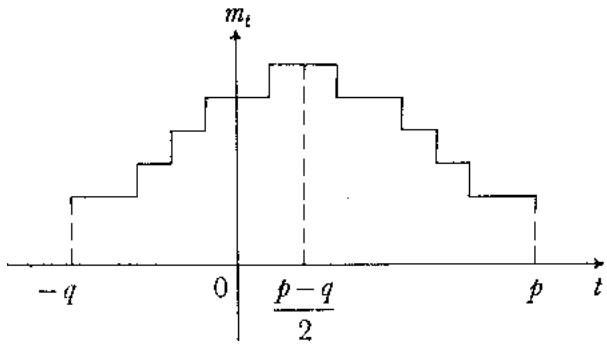
\includegraphics[keepaspectratio]{images/part001_39d2730e.jpg}}

（§1，第 2 节，命题 2）。由此可得：\(\mathrm{V}^{\lambda + t\alpha} \neq 0\)，只要 \(p \geq t \geq p - (\lambda(H_{\alpha}) + 2p)\)，所以 \(p + q \geq \lambda(H_{\alpha}) + 2p\)。将这个结果应用于 \(-\alpha\)，得到

\[
p + q \geq \lambda (H _ {- \alpha}) + 2 q = - \lambda (H _ {\alpha}) + 2 q.
\]

因此 \(q - p = \lambda (H_{\alpha})\)，且 \(\lambda + t\alpha \in \mathcal{X}\)（当 \(p \geq t \geq -q\) 时），这证明了 (i)。

我们有 \(s_{\alpha}(\alpha) = -\alpha\)，且 \(s_{\alpha}(\mu) \in \mu + k\alpha\) 对所有 \(\mu \in \mathfrak{h}^*\) 成立。由于 W 使 \(\mathcal{X}\) 保持稳定（命题 2 的推论 2），\(s_{\alpha}\) 使 \(\{\lambda - q\alpha, \lambda - q\alpha + \alpha, \ldots, \lambda + p\alpha\}\) 保持稳定，并将 \(\lambda - q\alpha + u\alpha\) 映到 \(\lambda + p\alpha - u\alpha\)，其中对所有 \(u \in k\) 都成立。再次使用命题 2 的推论 2，可见 \(m_{-q + u} = m_{p - u}\)，其中 \(u \in [0, p + q]\) 为任意整数。这证明了 (ii)。

根据 §1，命题 2 的推论，\((X_{\alpha})_{\mathrm{V}}|\mathrm{V}^{\lambda +t\alpha}\) 在 \(t < (p - q) / 2\) 时是单射。现在 \((X_{\alpha})_{\mathrm{V}}\) 将 \(\mathrm{V}^{\lambda +t\alpha}\) 映到 \(\mathrm{V}^{\lambda +(t + 1)\alpha}\)。所以 \(m_{t + 1}\geq m_t\)，只要 \(t < (p - q) / 2\)。将 \(\alpha\) 换成 \(-\alpha\)，可见 \(m_{t + 1}\leq m_t\)，只要 \(t > (p - q) / 2\)。这证明了 (iii) 和 (iv)。

推论 1. 若 \(\lambda \in \mathcal{X}\) 且 \(\lambda (H_{\alpha})\geq 1\)，则 \(\lambda -\alpha \in \mathcal{X}\)。若 \(\lambda +\alpha \in \mathcal{X}\) 且 \(\lambda (H_{\alpha}) = 0\)，则 \(\lambda \in \mathcal{X}\) 且 \(\lambda -\alpha \in \mathcal{X}\)。

这立即由命题 3 (i) 得出。

推论 2. 设 \(\mu \in \mathrm{P}_{++}\) 且 \(\nu \in \mathrm{Q}_{+}\)。若 \(\mu + \nu \in \mathcal{X}\)，则 \(\mu \in \mathcal{X}\)。

写成 \(\nu = \sum_{\alpha \in \mathrm{B}} c_{\alpha}.\alpha\)，其中 \(c_{\alpha} \in \mathbf{N}\) 对所有 \(\alpha \in \mathrm{B}\) 成立。当 \(\sum_{\alpha \in \mathrm{B}} c_{\alpha} = 0\) 时推论显然成立；假设 \(\sum_{\alpha \in \mathrm{B}} c_{\alpha} > 0\)，并对 \(\sum_{\alpha \in \mathrm{B}} c_{\alpha}\) 作归纳。设 \((\cdot|\cdot)\) 是 \(\mathfrak{h}_{\mathbf{R}}^{*}\) 上 W-不变的非退化正对称双线性型。于是 \((\nu|\sum_{\alpha \in \mathrm{B}} c_{\alpha}.\alpha) > 0\)，所以存在 \(\beta \in \mathrm{B}\)，使得 \(c_{\beta} \geq 1\) 且 \((\nu|\beta) > 0\)，从而 \(\nu(H_{\beta}) \geq 1\)。由于 \(\mu \in \mathrm{P}_{++}\)，可得 \((\mu + \nu)(H_{\beta}) \geq 1\)。根据推论 1，\(\mu + (\nu - \beta) \in \mathcal{X}\)，于是只需应用归纳假设。

推论 3. 设 \(v \in V\) 是权为 \(\omega\) 的本原元。设 \(\Sigma\) 为满足 \(\alpha \in B\) 且 \(\omega(H_{\alpha}) = 0\) 的元素所成的集合。\(\mathfrak{g}\) 中直线 \(kv\) 的稳定子是抛物子代数 \(\mathfrak{p}_{\Sigma}\)，它对应于 \(\Sigma\)（§3，第 4 节，备注）。

必要时以 v 生成的 g-子模替换 V，于是可假设 V 是单模。设 s 为稳定子。我们有 \((\mathfrak{n}_{+})_{\mathrm{V}}v = 0\)，\((\mathfrak{h})_{\mathrm{V}}v \subset kv\)。设 \(\alpha \in B\) 满足 \(\omega(H_{\alpha}) = 0\)。我们有 \(\omega + \alpha \notin X\)，从而 \(\omega - \alpha \notin X\)（命题 3 (i)），因而 \((\mathfrak{g}^{-\alpha})_{\mathrm{V}}v = 0\)。前述结果说明 \(p_{\Sigma} \subset s\)。若 \(p_{\Sigma} \neq s\)，则 \(s = p_{\Sigma'}\)，其中 \(\Sigma'\) 是严格包含 \(\Sigma\) 的 B 的子集。设 \(\beta \in \Sigma' - \Sigma\)。于是 \(g^{-\beta}\) 稳定 kv，因而湮灭 v。但是，由于 \(\omega(H_{\beta}) > 0\)，这与命题 3 (iii) 矛盾。证毕。

P 的一个子集 \(\mathcal{X}\) 称为 R-饱和的，如果满足以下条件：对所有 \(\lambda \in \mathcal{X}\) 和所有 \(\alpha \in \mathrm{R}\)，有 \(\lambda - t\alpha \in \mathcal{X}\)，其中 \(t\) 遍历 0 与 \(\lambda(H_{\alpha})\) 之间的所有整数。由于 \(s_{\alpha}(\lambda) = \lambda - \lambda(H_{\alpha})\alpha\)，可见 P 的 R-饱和子集在 W 下稳定。设 \(\mathcal{Y} \subset \mathrm{P}\)。\(\lambda\) 是 \(\mathcal{Y}\) 的一个元素，在 \(\mathcal{Y}\) 中称为 R-极值元，如果对所有 \(\alpha \in \mathrm{R}\)，都有 \(\lambda + \alpha \notin \mathcal{Y}\) 或 \(\lambda - \alpha \notin \mathcal{Y}\)。

命题 4. 设 \(\mathrm{V}\) 是有限维 \(\mathfrak{g}\)-模，\(d\) 是满足 \(\geq 1\) 的整数。\(\mathrm{V}\) 中重数 \(\geq d\) 的权的集合是 R-饱和的。

这立即由命题 3 得出。

命题 5. 设 V 是有限维单 g-模，\(\omega\) 是其最高权，X 是其权集。取双线性型 \((\cdot|\cdot)\)，它定义在 \(h_{R}^{*}\) 上，且 W-不变、非退化、正定；并令 \(\lambda\mapsto\|\lambda\|=(\lambda|\lambda)^{1/2}\) 为相应的范数。

\begin{enumerate}
\def\labelenumi{(\roman{enumi})}
\item
  \(\mathcal{X}\) 是包含 \(\omega\) 的 P 的最小 R-饱和子集。
\item
  \(\mathcal{X}\) 的 R-极值元正是 \(\omega\) 在 W 下的变换。
\item
  若 \(\mu \in \mathcal{X}\)，则 \(\| \mu \| \leq \| \omega \|\)。此外，若 \(\mu \neq \omega\)，则 \(\| \mu + \rho \| < \| \omega + \rho \|\)。若 \(\mu\) 不是 \(\mathcal{X}\) 中的 R-极值元，则 \(\| \mu \| < \| \omega \|\)。
\item
  我们有 \(\mathcal{X} = \mathrm{W.}(\mathcal{X}\cap \mathrm{P}_{++})\)。其中，\(\lambda\) 是 \(\mathrm{P}_{++}\) 中的元素；其属于 \(\mathcal{X}\cap \mathrm{P}_{++}\) 当且仅当 \(\omega -\lambda \in \mathrm{Q}_{+}\)。
\item
  设 \(\mathcal{X}'\) 是包含 \(\omega\) 的 P 的最小 R-饱和子集。我们有 \(\mathcal{X}' \subset \mathcal{X}\)（命题 4）。假设 \(\mathcal{X} \neq \mathcal{X}'\)。设 \(\lambda\) 是 \(\mathcal{X} - \mathcal{X}'\) 的极大元。由于 \(\lambda \neq \omega\)，存在 \(\alpha \in B\)，使得 \(\lambda + \alpha \in \mathcal{X}\)。按命题 3 引入 \(p\) 和 \(q\)。由于 \(\lambda\) 是 \(\mathcal{X} - \mathcal{X}'\) 中的极大元，\(\lambda + p\alpha \in \mathcal{X}'\)。根据命题 3 (ii)，\(\lambda - q\alpha \in \mathcal{X}'\)，因为 \(\mathcal{X}'\) 在 W 下稳定。因此，有 \(\lambda + u\alpha \in \mathcal{X}'\)，其中 \(u\) 遍历区间 \([-q, p]\) 中的每个整数。这与 \(\lambda \notin \mathcal{X}'\) 矛盾，从而证明了 (i)。
\item
  显然，\(\omega\) 是 \(\mathcal{X}\) 中的 R-极值元；因此它在 W 下的变换也都是 \(\mathcal{X}\) 中的 R-极值元。设 \(\lambda\) 是 \(\mathcal{X}\) 中的 R-极值元；我们将证明 \(\lambda \in \mathrm{W}.\omega\)。由于存在 \(w \in \mathrm{W}\)，使得 \(w\lambda \in \mathrm{P}_{++}\)（第 VI 章，§1，第 10 节），不妨设 \(\lambda \in \mathrm{P}_{++}\)。设 \(\alpha \in \mathrm{B}\)；按命题 3 引入 \(p\) 和 \(q\)。由于 \(\lambda\) 是 R-极值元，\(p = 0\) 或 \(q = 0\)。由于
\end{enumerate}

\[
q - p = \lambda (H _ {\alpha}) \geq 0,
\]

不可能有 \(p > 0\)。因此 \(p = 0\) 且 \(\lambda = \omega\)。

\begin{enumerate}
\def\labelenumi{(\roman{enumi})}
\setcounter{enumi}{2}
\tightlist
\item
  设 \(\mu \in \mathcal{X} \cap \mathrm{P}_{++}\)。则 \(\omega + \mu \in \mathrm{P}_{++}\) 且 \(\omega - \mu \in \mathrm{Q}_+\)（§6，第 1 节，命题 1），所以 \(0 \leq (\omega - \mu|\omega + \mu) = (\omega|\omega) - (\mu|\mu)\)；从而 \((\mu|\mu) \leq (\omega|\omega)\)，利用 Weyl 群可将此结论推广到所有 \(\mu \in \mathcal{X}\)。如果 \(\mu \in \mathcal{X} - \{\omega\}\)，
\end{enumerate}

\[
\begin{array}{c} (\mu + \rho | \mu + \rho) = (\mu | \mu) + 2 (\mu | \rho) + (\rho | \rho) \leq (\omega | \omega) + 2 (\mu | \rho) + (\rho | \rho) \\ = (\omega + \rho | \omega + \rho) - 2 (\omega - \mu | \rho). \end{array}
\]

现在 \(\omega - \mu = \sum_{\alpha \in \mathrm{B}} n_{\alpha} \alpha\)，其中整数 \(n_{\alpha} \geq 0\) 不全为零，所以 \((\omega - \mu | \rho) > 0\)，因为 \((\rho | \alpha) > 0\) 对所有 \(\alpha \in \mathrm{B}\) 都成立（第 VI 章，§1，第 10 节，命题 29 (iii)）。若 \(\mu\) 不是 \(\mathcal{X}\) 中的 R-极值元，则存在 \(\alpha \in \mathrm{R}\)，使得 \(\mu + \alpha \in \mathcal{X}\) 且 \(\mu - \alpha \in \mathcal{X}\)；于是

\[
\| \mu \| <   \sup (\| \mu + \alpha \|, \| \mu - \alpha \|) \leq \sup _ {\lambda \in \mathcal {X}} \| \lambda \|
\]

而根据前述结果，这个上界是 \(\|\omega\|\)。

\begin{enumerate}
\def\labelenumi{(\roman{enumi})}
\setcounter{enumi}{3}
\tightlist
\item
  根据第 VI 章，§1，第 10 节，我们有 \(\mathcal{X} = \mathrm{W.}(\mathcal{X}\cap \mathrm{P}_{++})\)。若 \(\lambda \in \mathcal{X}\)，则 \(\omega -\lambda \in \mathrm{Q}_{+}\)（§6，第 1 节，命题 1）。若 \(\lambda \in \mathrm{P}_{++}\) 且 \(\omega -\lambda \in \mathrm{Q}_{+}\)，则 \(\lambda \in \mathcal{X}\)（命题 3 的推论 2）。
\end{enumerate}

推论。设 X 是 P 的有限 R-饱和子集。存在一个权集为 X 的有限维 g-模。

由于 \(\mathcal{X}\) 在 W 下稳定，\(\mathcal{X}\) 是包含 \(\mathcal{X} \cap \mathrm{P}_{++}\) 的最小 R-饱和集。根据命题 5 (i)，\(\mathcal{X}\) 是 \(\bigoplus_{\lambda \in \mathcal{X} \cap \mathrm{P}_{++}} \mathrm{E}(\lambda)\) 的权集。

备注 2. 回顾一下（第 VI 章，§1，第 6 节，命题 17 的推论 3），存在唯一的 \(w_0\)，它是 \(\mathrm{W}\) 中将 \(\mathrm{B}\) 变为 \(-\mathrm{B}\) 的元素；我们有 \(w_0^2 = 1\)。并且 \(-w_0\) 保持 \(\mathrm{P}\) 上的序关系。记 \(\mathrm{V}\) 为有限维单 \(\mathfrak{g}\)-模，\(\omega\) 为其最高权。则 \(w_0(\omega)\) 是 \(\mathrm{V}\) 的最低权，且其重数为 1。

\subsection{极小权}

命题 6. 设 \(\lambda \in \mathrm{P}\)，\(\mathcal{X}\) 是包含 \(\lambda\) 的 P 的最小 R-饱和子集。取如命题 5 中的范数 \(\| \cdot \|\)。以下条件等价：

\begin{enumerate}
\def\labelenumi{(\roman{enumi})}
\item
  \(\mathcal{X} = \mathrm{W}.\lambda\) ;
\item
  \(\mathcal{X}\) 的所有元素具有相同的范数；
\item
  对所有 \(\alpha \in \mathrm{R}\)，都有 \(\lambda(H_{\alpha}) \in \{0,1,-1\}\)。
\end{enumerate}

P 的每个非空 R-饱和子集都包含一个满足上述条件的元素 \(\lambda\)。

引入条件：

（ii'）对所有 \(\alpha \in \mathrm{R}\)，设 \(t\) 为介于 0 与 \(\lambda(H_{\alpha})\) 之间的任一整数，

\[
\| \lambda - t \alpha \| \geq \| \lambda \|.
\]

\begin{enumerate}
\def\labelenumi{(\roman{enumi})}
\tightlist
\item
  \(\Longrightarrow\) (ii) \(\Longrightarrow\) (ii')：显然。
\end{enumerate}

\((\mathrm{ii}^{\prime}) \Longrightarrow (\mathrm{iii})\)：假设条件 \((\mathrm{ii}^{\prime})\) 满足。设 \(\alpha \in \mathrm{R}\)。我们有 \(\| \lambda \| = \| \lambda - \lambda (H_{\alpha})\alpha \|\)，所以有 \(\| \lambda - t\alpha \| < \| \lambda \|\)，其中 \(t\) 严格位于 0 与 \(\lambda (H_{\alpha})\) 之间；因此不存在这样的整数，从而 \(|\lambda (H_{\alpha})| \leq 1\)。

\begin{enumerate}
\def\labelenumi{(\roman{enumi})}
\setcounter{enumi}{2}
\tightlist
\item
  \(\Longrightarrow\) (i)：假设条件 (iii) 满足。设 \(w \in W\) 且 \(\alpha \in R\)。则 \((w\lambda)(H_{\alpha}) = \lambda(H_{w^{-1}\alpha}) \in \{0,1,-1\}\)；因此，若 t 是介于 0 与 \((w\lambda)(H_{\alpha})\) 之间的整数，则 \(w\lambda - t\alpha\) 等于 \(w\lambda\) 或 \(s_{\alpha}(w\lambda)\)。这证明 W. \(\lambda\) 是 R-饱和的，所以 X = W. \(\lambda\)。
\end{enumerate}

设 Y 是 P 的非空 R-饱和子集。Y 中存在一个范数最小的元素 \(\lambda\)。显然 \(\lambda\) 满足条件 (ii')，从而得到命题的最后一个断言。

命题 7. 设 V 是有限维单 g-模，X 是 V 的权集，\(\lambda\) 是 X 的最高元（参见命题 5 (i)）。命题 6 的条件 (i)、(ii) 和 (iii) 等价于：

\begin{enumerate}
\def\labelenumi{(\roman{enumi})}
\setcounter{enumi}{3}
\tightlist
\item
  对所有 \(\alpha \in \mathrm{R}\) 以及所有 \(x \in \mathfrak{g}^{\alpha}\)，都有 \((x_{\mathrm{V}})^2 = 0\)。
\end{enumerate}

若这些条件满足，则 V 的所有权的重数都为 1。

若 (i) 满足，则 \(X = W \cdot \lambda\)，且所有权都与 \(\lambda\) 具有相同的重数（命题 2 的推论 2），换言之，重数为 1。此外，若 \(w \in W\) 且 \(\alpha \in R\)，则 \(w\lambda + t\alpha\) 是 V 的权必有 \(|t| \leq 1\)。因此，若 \(x \in g^{\alpha}\)，

\[
(x _ {\mathrm{V}}) ^ {2} (\mathrm{V} ^ {w (\lambda)}) \subset \mathrm{V} ^ {w (\lambda) + 2 \alpha} = 0,
\]

所以 \((x_{\mathrm{V}})^2 = 0\)，这证明了 (i) \(\Longrightarrow\) (iv)。

反过来，假设 (iv) 满足。设 \(\alpha \in \mathrm{R}\)，并给 V 赋予 \(\mathfrak{sl}(2,k)\)-模结构，定义此结构的元素为 \(X_{\alpha}, X_{-\alpha}, H_{\alpha}\)，这些元素属于 \(\mathfrak{g}\)。将 (iv) 应用于 \(x = X_{\alpha}\)，可知 \(\mathfrak{sl}(2,k)\)-模 V 的权属于 \(\{0,1,-1\}\)（参见 §1，第 2 节，命题 2 的推论）。特别地，\(\lambda(H_{\alpha}) \in \{0,1,-1\}\)，所以 (iv) \(\Longrightarrow\) (iii)。

命题 8. 假设 g 是单的。以 \(\alpha_{1},\ldots,\alpha_{l}\) 表示 B 的元素。设 \(\varpi_{1},\ldots,\varpi_{l}\) 是相应的基本权。设 \(H = n_{1}H_{\alpha_{1}} + \cdots + n_{l}H_{\alpha_{l}}\) 是 \(R^{\vee}\) 的最高根，J 是这样的 \(i \in \{1,\ldots,l\}\) 的集合：满足 \(n_{i} = 1\)。设 \(\lambda \in P_{++} - \{0\}\)。则命题 6 的条件 (i)、(ii) 和 (iii) 分别等价于以下每个条件：

\begin{enumerate}
\def\labelenumi{(\alph{enumi})}
\setcounter{enumi}{21}
\tightlist
\item
  \(\lambda(H)=1;\)
\end{enumerate}

\begin{enumerate}
\def\labelenumi{(\roman{enumi})}
\setcounter{enumi}{5}
\tightlist
\item
  存在 \(i \in \mathrm{J}\)，使得 \(\lambda = \varpi_i\)。
\end{enumerate}

\(\varpi_{i}\)（其中 \(i \in J\)）在 P(R) 中构成 P(R)/Q(R) 的非零元素的一个代表系。

设 \(\lambda = u_{1}\varpi_{1} + \cdots + u_{l}\varpi_{l}\)，其中 \(u_{1}, \ldots, u_{l}\) 是满足 \(\geq 0\) 且不全为零的整数。则 \(\lambda(H) = u_{1}n_{1} + \cdots + u_{l}n_{l}\)，且 \(n_{1} \geq 1, \ldots, n_{l} \geq 1\)，这立即给出 (v) 与 (vi) 的等价性。另一方面，\(\lambda(H) = \sup_{\alpha \in \mathrm{R}_{+}} \lambda(H_{\alpha})\)，且 \(\lambda(H) > 0\)，因为 \(\lambda\) 是 \(P_{++}\) 的非零元素。因此，条件 (v) 等价于条件 \(\lambda(H_{\alpha}) \in \{0, 1\}\) 对所有 \(\alpha \in R\) 成立，换言之，等价于命题 6 的条件 (iii)。

命题的最后一个断言由第 VI 章，§2，第 3 节，命题 6 的推论得出。

定义 1. 假设 \(\mathfrak{g}\) 是单的。\((\mathfrak{g},\mathfrak{h})\) 的极小权是 \(\mathrm{P}_{++} - \{0\}\) 中满足命题 6、7 和 8 的等价条件 (i)、(ii)、(iii)、(iv)、(v) 和 (vi) 的元素。

备注。假设 g 是单的。设 \(\Sigma^{\prime\vee}\) 是仿射 Weyl 群 \(\mathrm{W}_{a}(\mathrm{R}^{\vee})\) 的 Coxeter 图。回顾一下，\(\Sigma^{\prime\vee}\) 的顶点是 Coxeter 图 \(\Sigma^{\vee}\)（即 \(\mathrm{W}(\mathrm{R}^{\vee})\) 的 Coxeter 图）的顶点，再加上一个补充顶点 0。群 \(\mathrm{A}(\mathrm{R}^{\vee})\) 作用于 \(\Sigma^{\prime\vee}\)，并固定 0。群 \(\mathrm{Aut}(\Sigma^{\prime\vee})\) 典则同构于 \(\mathrm{A}(\mathrm{R}^{\vee})/\mathrm{W}(\mathrm{R}^{\vee})\) 与群 \(\Gamma_{C}\) 的半直积（参见第 VI 章，§2，第 3 节以及第 VI 章，§4，第 3 节）；显然 \((\operatorname{Aut} \Sigma'^{\vee})(0) = \Gamma_C(0)\)；并且 \(\Gamma_C(0)\) 由 0 以及 \(\Sigma^{\vee}\) 中与 \(\varpi_i\)（其中 \(i \in \mathbf{J}\)）对应的顶点组成（参见第 VI 章，§2，命题 5 以及第 3 节的备注 1）。总之，极小权是与 \(\Sigma^{\vee}\) 中可由 \(\operatorname{Aut}(\Sigma'^{\vee})\) 的某个元素作用于 0 而得到的顶点相对应的基本权。

采用第 VI 章图版 I 至 IX 的记号，由前述结果可推出，极小权如下：

对于 \(A_{l}\) 型（\(l \geq 1\)）：\(\varpi_{1}, \ldots, \varpi_{l}\)。

对于 \(B_{l}\) 型（\(l \geq 2\)）：\(\varpi_{l}\)。

对于 \(C_{l}\) 型（\(l \geq 2\)）：\(\varpi_{1}\)。

对于 \(D_{l}\) 型（\(l \geq 3\)）：\(\varpi_{1}, \varpi_{l-1}, \varpi_{l}\)。

对于 \(E_{6}\) 型：\(\varpi_{1}, \varpi_{6}\)。

对于 \(\mathrm{E}_7\) 型：\(\varpi_7\)。

对于 \(E_{8}, F_{4}, G_{2}\) 型，不存在极小权。

\subsection{g-模的张量积}

设 \(\mathrm{E},\mathrm{F}\) 为 \(\mathfrak{g}\)-模。对于所有 \(\lambda, \mu \in \mathfrak{h}^*\)，有 \(\mathrm{E}^\lambda \otimes \mathrm{F}^\mu \subset (\mathrm{E} \otimes \mathrm{F})^{\lambda + \mu}\)（第 VII 章，§1，第 1 节，命题 2 (ii)）。若 \(\mathrm{E}\) 和 \(\mathrm{F}\) 是有限维的，则 \(\mathrm{E} = \sum_{\lambda \in \mathrm{P}} \mathrm{E}^\lambda\) 且 \(\mathrm{F} = \sum_{\mu \in \mathrm{P}} \mathrm{F}^\mu\)；因此，

\[
(\mathrm{E} \otimes \mathrm{F}) ^ {\nu} = \sum_ {\lambda , \mu \in \mathrm{P}, \lambda + \mu = \nu} \mathrm{E} ^ {\lambda} \otimes \mathrm{F} ^ {\mu}.
\]

换言之，赋予 \(E \otimes F\) 其 P 型分次后，它是分次向量空间 E 和 F 的分次张量积。

命题 9. 设 E、F 是有限维单 g-模，最高权分别为 \(\lambda,\mu\)。

\begin{enumerate}
\def\labelenumi{(\roman{enumi})}
\item
  \(\mathrm{E} \otimes \mathrm{F}\) 中最高权为 \(\lambda + \mu\) 的分量是一个单子模，由 \((\mathrm{E} \otimes \mathrm{F})^{\lambda + \mu} = \mathrm{E}^{\lambda} \otimes \mathrm{F}^{\mu}\) 生成。
\item
  \(\mathrm{E} \otimes \mathrm{F}\) 的任意单子模的最高权都 \(\leq \lambda + \mu\)（参见 §9，命题 2）。
\end{enumerate}

若 \(\alpha, \beta \in \mathrm{P}\) 且 \(\mathrm{E}^{\alpha} \otimes \mathrm{F}^{\beta} \neq 0\)，则 \(\alpha \leq \lambda\) 且 \(\beta \leq \mu\)。因此，\((\mathrm{E} \otimes \mathrm{F})^{\lambda + \mu}\) 等于 \(\mathrm{E}^{\lambda} \otimes \mathrm{F}^{\mu}\)，从而维数为 1，而 \(\lambda + \mu\) 是 \(\mathrm{E} \otimes \mathrm{F}\) 的最高权。 \(\mathrm{E}^{\lambda} \otimes \mathrm{F}^{\mu}\) 的每个非零元素都是本原元。根据 §6 第 2 节的命题 4，\(\mathrm{E} \otimes \mathrm{F}\) 中最高权为 \(\lambda + \mu\) 的同构型分支的长度为 1。

备注。保留命题 9 的记号。设 C 是 \(E \otimes F\) 中最高权为 \(\lambda + \mu\) 的同构型分支。则 C 只依赖于 E 和 F，而不依赖于 h 和基 B 的选择。换言之，设 \(h'\) 是 g 的一个分裂嘉当子代数，\(R'\) 是 \((\mathfrak{g}, \mathfrak{h}')\) 的根系，\(B'\) 是 \(R'\) 的一个基；设 \(\lambda', \mu'\) 是 E、F 关于 \(h'\) 和 \(B'\) 的最高权；设 \(C'\) 是 \(E \otimes F\) 中最高权为 \(\lambda' + \mu'\) 的同构型分支；则 \(C' = C\)。事实上，为证明这一点，可以通过扩张基域假设 k 是代数闭域。于是存在 \(s \in \operatorname{Aut}_{e}(\mathfrak{g})\)，将 \(h\) 映到 \(h'\)，将 R 映到 \(R'\)，将 B 映到 \(B'\)。设 \(S \in \mathbf{SL}(E \otimes F)\) 具有第 1 节命题 2 中的性质。于是 \(\mathrm{S}((\mathrm{E} \otimes \mathrm{F})^{\lambda + \mu}) = (\mathrm{E} \otimes \mathrm{F})^{\lambda' + \mu'}\)，且 \(\mathrm{S}(\mathrm{C}) = \mathrm{C}\)。因此 \((\mathrm{E} \otimes \mathrm{F})^{\lambda' + \mu'} \subset \mathrm{C}' \cap \mathrm{S}(\mathrm{C}) = \mathrm{C}' \cap \mathrm{C}\)，所以 \(C' = C\)。这样，两个有限维单 g-模的同构类可典则地确定第三个同构类；换言之，我们在有限维单 g-模的同构类集合 \(S_{g}\) 上定义了一个复合律。在此结构下，\(S_{g}\) 典则同构于加法幺半群 \(P_{++}\)。

推论 1. 设 \((\varpi_{\alpha})_{\alpha \in \mathrm{B}}\) 是关于 B 的基本权族。设 \(\lambda = \sum_{\alpha \in \mathrm{B}} m_{\alpha} \varpi_{\alpha} \in \mathrm{P}_{++}\)。对于所有 \(\alpha \in \mathrm{B}\)，设 \(\mathrm{E}_{\alpha}\) 是单 \(\mathfrak{g}\)-模，其最高权为 \(\varpi_{\alpha}\)。在 \(\mathfrak{g}\)-模 \(\bigotimes_{\alpha \in \mathrm{B}} (\bigotimes^{m_{\alpha}} \mathrm{E}_{\alpha})\) 中，最高权为 \(\lambda\) 的同构型分支长度为 1。

这由命题 9 对 \(\sum_{\alpha \in \mathrm{B}}m_{\alpha}\) 作归纳得到。

推论 2. 假设 k 是 R、C 或非离散完备超度量域。设 G 是李代数为 g 的李群。假设对于 g 的任意基本表示 \(\rho\)，都存在 G 的一个解析线性表示 \(\rho'\)，使得 \(\rho = \mathrm{L}(\rho')\)。那么对于 g 的任意有限维线性表示 \(\pi\)，都存在 G 的一个解析线性表示 \(\pi'\)，使得 \(\pi = \mathrm{L}(\pi')\)。

使用推论 1 的记号。存在一个 G 的表示 \(\sigma\)，作用在 \(X = \bigotimes_{\alpha \in B} (\bigotimes^{m_{\alpha}} E_{\alpha})\) 上，使得 \(L(\sigma)\) 对应于 X 的 \(\mathfrak{g}\)-模结构（第 III 章，§3，第 11 节，命题 41 的推论 3）。设 C 是 X 中最高权为 \(\lambda\) 的同构型分支。根据第 III 章，§3，第 11 节，命题 40，只需证明 C 在 \(\sigma(G)\) 下稳定。设 \(g \in G\)，且 \(\varphi = \operatorname{Ad}(g)\)。则 \(\sigma(g)a_X \sigma(g)^{-1} = (\varphi(a))_X\) 对所有 \(a \in \mathfrak{g}\) 成立。另一方面，\(\varphi\) 是 \(\mathfrak{g}\) 的一个自同构，将 \(\mathfrak{h}\) 映到 \(\mathfrak{h}'\)，将 R 映到 \(R' = R(\mathfrak{g}, \mathfrak{h}')\)，将 B 映到 \(B'\)，它是 \(R'\) 的一个基，并将 \(\varpi_{\alpha}\) 映到 \(\varpi_{\alpha}'\)，即 \(E_{\alpha}\) 关于 \(\mathfrak{h}'\) 和 \(B'\) 的最高权（因为 \(\varphi\) 将 \(E_{\alpha}\) 变为一个 \(\mathfrak{g}\)-模，该模与 \(E_{\alpha}\) 同构）。因此 \(\varphi\) 将 \(\lambda\) 映到 \(\sum m_{\alpha} \varpi_{\alpha}'\)。根据上面的备注，\(\sigma(g)(C) = C\)。

命题 10. 设 \(\lambda, \mu \in \mathrm{P}_{++}\)。设 E、F、G 是单 \(\mathfrak{g}\)-模，其最高权分别为 \(\lambda, \mu, \lambda + \mu\)。设 \(\mathcal{X}\)（分别为 \(\mathcal{X}', \mathcal{X}''\)）是 E（分别为 F、G）的权集。则 \(\mathcal{X}'' = \mathcal{X} + \mathcal{X}'\)。

我们有 \(E = \bigoplus_{\nu \in P} E^{\nu}, F = \bigoplus_{\sigma \in P} F^{\sigma}\)，所以 \(E \otimes F\) 是下列各空间的直和

\[
(\mathrm{E} \otimes \mathrm{F}) ^ {\tau} = \sum_ {\nu + \sigma = \tau} \mathrm{E} ^ {\nu} \otimes \mathrm{F} ^ {\sigma}.
\]

根据命题 9，\(\mathbf{G}\) 可识别为一个 \(\mathfrak{g}\)-子模，并且它包含在 \(\mathrm{E} \otimes \mathrm{F}\) 中，因此 \(\mathcal{X}'' \subset \mathcal{X} + \mathcal{X}'\)。我们有 \(\mathrm{G}^{\tau} = \mathrm{G} \cap (\mathrm{E} \otimes \mathrm{F})^{\tau}\)，只需证明：对于 \(\nu \in \mathcal{X}\) 和 \(\sigma \in \mathcal{X}'\)，有 \(\mathrm{G} \cap (\mathrm{E} \otimes \mathrm{F})^{\nu + \sigma} \neq 0\)。设 \((e_1, \ldots, e_n)\)（分别为 \((f_1, \ldots, f_p))\) 是 \(\mathrm{E}\)（分别为 \(\mathrm{F}\)）的一个基，其中每个基向量属于某个 \(\mathrm{E}^\nu\)（分别为 \(\mathrm{F}^\sigma\)），并且 \(e_1 \in \mathrm{E}^\lambda\)（分别为 \(f_1 \in \mathrm{F}^\mu\)）。\(e_i \otimes f_j\) 构成 \(\mathrm{E} \otimes \mathrm{F}\) 的一个基。假设要证明的结论不成立。则存在一对 \((i,j)\)，使得每个 \((i,j)\) 号坐标在 \(\mathrm{G}\) 的每个元素中都为零。设 \(\mathrm{U}\) 是 \(\mathfrak{g}\) 的包络代数，\(\mathrm{U}'\) 是 \(\mathrm{U}\) 的对偶，\(c\) 是 \(\mathrm{U}\) 的余积。对于所有 \(u \in \mathrm{U}\)，令 \(x_i(u)\)（分别为 \(y_j(u)\)）为 \(u(e_1)\)（分别为 \(u(f_1)\)）的 \(i\)（分别为 \(j\)）号坐标；令 \(z_{ij}(u)\) 为编号为 \((i,j)\) 的 \(u(e_1 \otimes f_1)\) 的坐标。于是 \(x_i, y_j, z_{ij} \in \mathrm{U}'\)。现在 \(e_1\) 生成 \(\mathfrak{g}\)-模 \(\mathrm{E}\)，所以 \(x_i \neq 0\)，同样 \(y_j \neq 0\)。根据 \(\mathfrak{g}\)-模 \(\mathrm{E} \otimes \mathrm{F}\) 的定义（第 I 章，§3，第 2 节），若 \(c(u) = \sum u_s \otimes u_s'\)，则有

\[
z _ {i j} (u) = \sum_ {s} x _ {i} (u _ {s}). y _ {j} (u _ {s} ^ {\prime}) = \langle c (u), x _ {i} \otimes y _ {j} \rangle .
\]

换言之，\(z_{ij}\) 是 \(x_{i}\) 与 \(y_{j}\) 在代数 \(U'\) 中的乘积。但这个代数是整环（第 II 章，§1，第 5 节，命题 10），所以 \(z_{ij} \neq 0\)。由于 \(u(e_{1} \otimes f_{1}) \in \mathrm{G}\) 对所有 \(u \in U\) 成立，这就矛盾了。

\subsection{g-模的对偶}

设 E、F 为 g-模。回顾一下（第 I 章，§3，第 3 节），\(\operatorname{Hom}_{k}(\operatorname{E},\operatorname{F})\) 具有典则的 g-模结构。设 \(\varphi\) 是权为 \(\lambda\) 的 \(\operatorname{Hom}_{k}(\operatorname{E},\operatorname{F})\) 中的元素。若 \(\mu \in h^{*}\)，则 \(\varphi(\operatorname{E}^{\mu}) \subset \operatorname{F}^{\lambda + \mu}\)（第 VII 章，§1，第 1 节，命题 2 (ii)）。因此，若 E 和 F 是有限维的，则权为 \(\lambda\) 的 \(\operatorname{Hom}_{k}(\operatorname{E},\operatorname{F})\) 中的元素，正是《代数》第 II 章 §11 第 2 节定义 4 意义下的次数为 \(\lambda\) 的分次同态。

命题 11. 设 E 是有限维 g-模，并考虑 g-模 \(E^{*} = \operatorname{Hom}_{k}(E, k)\)。

\begin{enumerate}
\def\labelenumi{(\roman{enumi})}
\item
  元素 \(\lambda \in \mathrm{P}\) 是 \(\mathrm{E}^*\) 的权，当且仅当 \(-\lambda\) 是 \(\mathrm{E}\) 的权；并且 \(\lambda\) 在 \(\mathrm{E}^*\) 中的重数等于 \(-\lambda\) 在 \(\mathrm{E}\) 中的重数。
\item
  若 \(\mathrm{E}\) 是最高权为 \(\omega\) 的单模，则 \(\mathrm{E}^*\) 是最高权为 \(-w_0(\omega)\) 的单模（参见第 2 节的备注 2）。
\end{enumerate}

把 k 看作元素权为 0 的平凡 g-模。根据上面的论述，\(E^{*}\) 中权为 \(\lambda\) 的元素，是从 E 到 k 的同态；它们在 \(E^{\mu}\) 上为零，只要 \(\mu \neq -\lambda\)。这证明了 (i)。若 E 是单模，则 \(E^{*}\) 也是单模（第 I 章，§3，第 3 节），最后一个断言由第 2 节的备注 2 得出。

备注。1) 设 E、E* 如命题 11 中，并设 \(\sigma \in \mathrm{Aut}(\mathfrak{g},\mathfrak{h})\) 满足，在 §5 第 1 节的记号下，\(\varepsilon (\sigma) = -w_0\)（§5，第 2 节，命题 2）。设 \(\rho ,\rho^{\prime}\) 是与 E、E* 相关的 \(\mathfrak{g}\) 表示。则 \(\rho \circ \sigma\) 是 \(\mathfrak{g}\) 的一个单表示，其最高权为 \(-w_{0}(\omega)\)，所以 \(\rho \circ \sigma\) 与 \(\rho^{\prime}\) 等价。

\begin{enumerate}
\def\labelenumi{\arabic{enumi})}
\setcounter{enumi}{1}
\tightlist
\item
  假设 \(w_{0} = -1\)。那么对于任意有限维 g-模 E，E 都同构于 \(E^{*}\)。回顾一下，若 g 是单的，则在以下情形中 \(w_{0} = -1\)：g 为 \(A_{1}, B_{l} (l \geq 2)\) 型、\(C_{l} (l \geq 2)\) 型、\(D_{l} (l \text{ even } \geq 4)\) 型，或 \(E_{7}, E_{8}, F_{4}, G_{2}\) 型（第 VI 章，图版）。
\end{enumerate}

引理 2. 令 \(h^0 = \sum_{\alpha \in \mathrm{R}_{+}} H_\alpha\)。则 \(h^0 = \sum_{\alpha \in \mathrm{B}} a_\alpha H_\alpha\)，其中 \(a_\alpha\) 是满足 \(\geq 1\) 的整数。设 \((b_\alpha)_{\alpha \in \mathrm{B}}, (c_\alpha)_{\alpha \in \mathrm{B}}\) 是满足 \(b_\alpha c_\alpha = a_\alpha\) 对所有 \(\alpha \in \mathrm{B}\) 成立的标量族。置 \(x = \sum_{\alpha \in \mathrm{B}} b_\alpha X_\alpha, y = \sum_{\alpha \in \mathrm{B}} c_\alpha X_{-\alpha}\)。存在一个同态 \(\varphi\)，从 \(\mathfrak{sl}(2,k)\) 到 \(\mathfrak{g}\)，使得 \(\varphi(H) = h^0, \varphi(X_+) = x, \varphi(X_-) = y\)。

事实 \(a_{\alpha}\) 是满足 \(\geq 1\) 的整数，是因为 \((H_{\alpha})_{\alpha \in \mathrm{B}}\) 是根系 \((H_{\alpha})_{\alpha \in \mathrm{B}}\) 的一个基（参见第 VI 章，§1，第 5 节，备注 5）。我们有：

\[
\alpha (h ^ {0}) = 2\tag{1}
\]

对所有 \(\alpha \in \mathrm{B}\) 都成立（第 VI 章，§1，第 10 节，命题 29 的推论），因此

\[
[ h ^ {0}, x ] = \sum_ {\alpha \in \mathrm{B}} b _ {\alpha} \alpha (h ^ {0}) X _ {\alpha} = 2 x\tag{2}
\]

\[
[ h ^ {0}, y ] = \sum_ {\alpha \in \mathrm{B}} c _ {\alpha} (- \alpha (h ^ {0})) X _ {- \alpha} = - 2 y.\tag{3}
\]

另一方面，

\[
[ x, y ] = \sum_ {\alpha , \beta \in \mathrm{B}} b _ {\alpha} c _ {\beta} [ X _ {\alpha}, X _ {- \beta} ] = \sum_ {\alpha \in \mathrm{B}} b _ {\alpha} c _ {\alpha} [ X _ {\alpha}, X _ {- \alpha} ] = - \sum_ {\alpha \in \mathrm{B}} a _ {\alpha} H _ {\alpha} = - h ^ {0},\tag{4}
\]

从而同态 \(\varphi\) 存在。

命题 12. 设 E 是有限维单 g-模，\(\omega\) 是其最高权，B 是 E 上 g-不变双线性型的向量空间。设 m 是整数 \(\sum_{\alpha\in\mathrm{R}_{+}}\omega(H_{\alpha})\)，从而 m/2 是 \(\omega\) 关于 B 的坐标之和（第 VI 章，§1，第 10 节，命题 29 的推论）。设 \(w_{0}\) 是满足 \(w_{0}(B) = -B\) 的 W 中的元素。

\begin{enumerate}
\def\labelenumi{(\roman{enumi})}
\item
  若 \(w_0(\omega) \neq -\omega\)，则 \(\mathcal{B} = 0\)。
\item
  假设 \(w_{0}(\omega) = -\omega\)。则 B 的维数为 1，且 B 的每个非零元素都是非退化的。若 m 为偶数（分别为奇数），则 B 的每个元素都是对称的（分别为交错的）。
\end{enumerate}

\begin{enumerate}
\def\labelenumi{\alph{enumi})}
\item
  设 \(\Phi \in \mathcal{B}\)。令 \(\varphi\) 为从 E 到 \(\mathrm{E}^*\) 的映射，对 \(x, y \in \mathrm{E}\) 定义为 \(\varphi(x)(y) = \Phi(x, y)\)；它是 \(\mathfrak{g}\)-模同态。若 \(\Phi \neq 0\)，则 \(\varphi \neq 0\)，所以根据 Schur 引理，\(\varphi\) 是同构，从而 \(\Phi\) 非退化。因此，\(\mathfrak{g}\)-模 E 同构于 \(\mathfrak{g}\)-模 \(\mathrm{E}^*\)，故 \(w_0(\omega) = -\omega\)。至此证明了 (i)。
\item
  从现在起假设 \(w_{0}(\omega) = -\omega\)。则 E 同构于 \(E^{*}\)。向量空间 B 同构于 \(\operatorname{Hom}_{\mathfrak{g}}(\mathrm{E}, \mathrm{E}^{*})\)，从而同构于 \(\operatorname{Hom}_{\mathfrak{g}}(\mathrm{E}, \mathrm{E})\)，后者的维数为 1（§6，第 1 节，命题 1 (iii)）。因此 \(\dim B = 1\)。根据 a)，B 的每个非零元素 \(\Phi\) 都是非退化的。令 \(\Phi_{1}(x, y) = \Phi(y, x)\)，其中 \(x, y \in E\)。由前述结果，存在 \(\lambda \in k\)，使得 \(\Phi_{1}(x, y) = \lambda \Phi(x, y)\) 对所有 \(x, y \in E\) 成立。于是 \(\Phi(y, x) = \lambda \Phi(x, y) = \lambda^{2} \Phi(y, x)\)，所以 \(\lambda^{2} = 1\) 且 \(\lambda = \pm 1\)。因此，\(\Phi\) 或者是对称的，或者是交错的。
\item
根据第 VII 章，§1，第 3 节，命题 9 (v)，\(E^{\lambda}\) 与 \(E^{\mu}\) 关于 \(\Phi\) 正交，只要 \(\lambda + \mu \neq 0\)。由于 \(\Phi\) 非退化，可知 \(E^{\omega}, E^{-\omega}\) 关于 \(\Phi\) 不正交。
\end{enumerate}

\(d\)）存在一个同态 \(\varphi\)，从 \(\mathfrak{sl}(2,k)\) 满射到 \(\mathfrak{g}\) 的某个子代数，并将 \(H\) 映到 \(\sum_{\alpha \in \mathrm{R}_{+}}H_{\alpha}\)（引理 2）。通过这个同态，把 E 看作一个 \(\mathfrak{sl}(2,k)\)-模。于是，\(\mathrm{E}^{\lambda}\) 的元素具有权 \(\lambda \left(\sum_{\alpha \in \mathrm{R}_{+}}H_\alpha\right)\)。若 \(\lambda \in \mathrm{P}\) 满足 \(\mathrm{E}^{\lambda} \neq 0\) 且 \(\lambda \neq \omega, \lambda \neq -\omega\)，则 \(-\omega < \lambda < \omega\)，所以

\[
- m = - \omega \left(\sum_ {\alpha \in \mathrm{R} _ {+}} H _ {\alpha}\right) <   \lambda \left(\sum_ {\alpha \in \mathrm{R} _ {+}} H _ {\alpha}\right) <   \omega \left(\sum_ {\alpha \in \mathrm{R} _ {+}} H _ {\alpha}\right) = m.
\]

令 \(G\) 为类型为 \(V(m)\) 的 \(\mathfrak{sl}(2, k)\)-模 \(E\) 的同构型分支。由上文，\(G\) 的长度为 1，且包含 \(E^{\omega}, E^{-\omega}\)。根据 \(c\)，\(\Phi\) 在 \(G\) 上的限制非零。根据 §1，第 3 项，备注 3，\(m\) 是偶数还是奇数，取决于这个限制是对称的还是交错的。鉴于 \(b\)，证毕。

定义 2. 若 g 的有限维不可约表示 \(\rho\) 在 E 上存在一个关于 \(\rho\) 不变的非退化对称（分别为交错）双线性型，则称该表示是正交型（分别为辛型）的。

\subsection{表示环}

设 \(\mathfrak{a}\) 是有限维李代数。设 \(\mathcal{F}_{\mathfrak{a}}\)（分别为 \(\mathfrak{S}_{\mathfrak{a}}\)）是有限维（分别为有限维单）\(\mathfrak{a}\)-模的同构类集合。设 \(\mathcal{R}(\mathfrak{a})\) 是自由阿贝尔群 \(\mathbf{Z}^{(\mathfrak{S}_{\mathfrak{a}})}\)。对于任意有限维单 \(\mathfrak{a}\)-模 E，以 {[}E{]} 表示其同构类。设 F 是有限维 \(\mathfrak{a}\)-模；设 \((\mathrm{F}_n,\mathrm{F}_{n - 1},\dots ,\mathrm{F}_0)\) 是 F 的 Jordan–Hölder 序列；则 \(\sum_{i = 1}^{n}[\mathrm{F}_i / \mathrm{F}_{i - 1}]\) 是 \(\mathcal{R}(\mathfrak{a})\) 中的元素，只依赖于 F，而不依赖于 Jordan–Hölder 序列的选择；我们将其记为 {[}F{]}。如果

\[
0 \longrightarrow \mathrm{F} ^ {\prime} \longrightarrow \mathrm{F} \longrightarrow \mathrm{F} ^ {\prime \prime} \longrightarrow 0
\]

是有限维 \(\mathfrak{a}\)-模的正合序列，则 \([\mathrm{F}] = [\mathrm{F}'] + [\mathrm{F}'']\)。

设 \(\mathrm{F}\) 是有限维半单 \(\mathfrak{a}\)-模；对于所有 \(\mathrm{E} \in \mathfrak{S}_{\mathfrak{a}}\)，设 \(n_{\mathrm{E}}\) 是 \(\mathrm{F}\) 中类型为 \(\mathrm{E}\) 的同构型分支的长度；则 \([\mathrm{F}] = \sum_{\mathrm{E} \in \mathfrak{S}_{\mathfrak{a}}} n_{\mathrm{E}}. \mathrm{E}\)。若 \(\mathrm{F}, \mathrm{F}'\) 是有限维半单 \(\mathfrak{a}\)-模，且 \([\mathrm{F}] = [\mathrm{F}']\)，则 \(\mathrm{F}\) 与 \(\mathrm{F}'\) 同构。

引理 3. 设 G 是用加法记号书写的阿贝尔群，\(\varphi : \mathcal{F}_{\mathfrak{a}} \to \mathrm{G}\) 是一个映射；略滥用记号，以 \(\varphi(\mathrm{F})\) 表示任意有限维模 F 的同构类在 \(\varphi\) 下的像，其中 F 是 \(\mathfrak{a}\)-模。假设对于任意正合序列

\[
0 \longrightarrow \mathrm{F} ^ {\prime} \longrightarrow \mathrm{F} \longrightarrow \mathrm{F} ^ {\prime \prime} \longrightarrow 0
\]

对于有限维 \(\mathfrak{a}\)-模，有 \(\varphi(\mathrm{F}) = \varphi(\mathrm{F}') + \varphi(\mathrm{F}'')\)。于是存在唯一的同态 \(\theta: \mathcal{R}(\mathfrak{a}) \to \mathrm{G}\)，使得 \(\theta([\mathrm{F}]) = \varphi(\mathrm{F})\) 对每个有限维 \(\mathfrak{a}\)-模 \(\mathrm{F}\) 成立。

存在唯一的同态 \(\theta\) 从 \(\mathcal{R}(\mathfrak{a})\) 到 G，使得对每个有限维单 a-模 E，都有 \(\theta([\mathrm{E}]) = \varphi(\mathrm{E})\)。设 F 是有限维 a-模，\((\mathrm{F}_{n}, \mathrm{F}_{n-1}, \ldots, \mathrm{F}_{0})\) 是 F 的 Jordan–Hölder 序列；若 \(n > 0\)，则对 n 作归纳可得

\[
\theta ([ \mathrm{F} ]) = \sum_ {i = 1} ^ {n} \theta ([ \mathrm{F} _ {i} / \mathrm{F} _ {i - 1} ]) = \sum_ {i = 1} ^ {n} \varphi (\mathrm{F} _ {i} / \mathrm{F} _ {i - 1}) = \varphi (\mathrm{F}).
\]

若 \(n = 0\)，则 \([\mathrm{F}] = 0\)，所以 \(\theta([\mathrm{F}]) = 0\)；另一方面，考察正合序列 \(0 \longrightarrow 0 \longrightarrow 0 \longrightarrow 0 \longrightarrow 0\)，可见 \(\varphi(0) = 0\)。

例。取 G = Z，且 \(\varphi(F) = \dim F\)。相应的从 \(\mathcal{R}(\mathfrak{a})\) 到 Z 的同态记为 dim。设 c 是一个维数为 1 的平凡 a-模的同构类，设 \(\psi\) 是由 \(n \mapsto nc\) 定义的同态，从 Z 到 \(\mathcal{R}(\mathfrak{a})\)。显然有

\(\dim \circ \psi = \operatorname{Id}_{\mathbf{Z}},\)

因此 \(\mathcal{R}(\mathfrak{a})\) 是 \(\operatorname{Kerdim}\) 与 \(\mathbf{Zc}\) 的直和。

引理 4. 在加法群 \(\mathcal{R}(\mathfrak{a})\) 上存在唯一的、关于加法可分配的乘法，使得 \([\mathrm{E}][\mathrm{F}] = [\mathrm{E}\otimes \mathrm{F}]\) 对所有有限维 \(\mathfrak{a}\)-模 E、F 成立。这样，\(\mathcal{R}(\mathfrak{a})\) 具有交换环的结构。维数为 1 的平凡 \(\mathfrak{a}\)-模的同构类是这个环的单位元。

唯一性显然。在 \(\mathcal{R}(\mathfrak{a}) = \mathbf{Z}^{(\mathfrak{S}_{\mathfrak{a}})}\) 上存在关于加法可分配的交换乘法，使得 \([E][F] = [E \otimes F]\) 对所有 \(E, F \in S_{a}\) 成立。设 \(E_{1}, E_{2}\) 是有限维 a-模，\(l_{1}\) 和 \(l_{2}\) 是它们的长度；我们证明 \([E_{1}][E_{2}] = [E_{1} \otimes E_{2}]\)，方法是对 \(l_{1} + l_{2}\) 作归纳。当 \(l_{1} + l_{2} \leq 2\) 时显然成立。另一方面，设 \(F_{1}\) 是 \(E_{1}\) 的一个既不为 0 也不为 \(E_{1}\) 的子模。于是

\[
[ \mathrm{F} _ {1} ] [ \mathrm{E} _ {2} ] = [ \mathrm{F} _ {1} \otimes \mathrm{E} _ {2} ] \text { and } [ \mathrm{E} _ {1} / \mathrm{F} _ {1} ] [ \mathrm{E} _ {2} ] = [ (\mathrm{E} _ {1} / \mathrm{F} _ {1}) \otimes \mathrm{E} _ {2} ]
\]

根据归纳假设。另一方面，\((\mathrm{E}_1\otimes \mathrm{E}_2) / (\mathrm{F}_1\otimes \mathrm{E}_2)\) 同构于 \((\mathrm{E}_1 / \mathrm{F}_1)\otimes \mathrm{E}_2\)。因此

\[
[ \mathrm{E} _ {1} ] [ \mathrm{E} _ {2} ] = ([ \mathrm{E} _ {1} / \mathrm{F} _ {1} ] + [ \mathrm{F} _ {1} ]). [ \mathrm{E} _ {2} ] = [ (\mathrm{E} _ {1} / \mathrm{F} _ {1}) \otimes \mathrm{E} _ {2} ] + [ \mathrm{F} _ {1} \otimes \mathrm{E} _ {2} ] = [ \mathrm{E} _ {1} \otimes \mathrm{E} _ {2} ],
\]

这就证明了我们的断言。立即可见，上面定义的乘法是结合的，所以 \(\mathcal{R}(\mathfrak{a})\) 具有交换环的结构。最后，显然维数为 1 的平凡 a-模的同构类是这个环的单位元。

引理 5. 存在唯一的对合自同构 \(\mathrm{X} \mapsto \mathrm{X}^*\)，定义在环 \(\mathcal{R}(\mathfrak{a})\) 上，使得 \([\mathrm{E}]^* = [\mathrm{E}^*]\) 对每个有限维 \(\mathfrak{a}\)-模 \(\mathrm{E}\) 成立。

唯一性显然。根据引理 3，存在一个同态 \(X \mapsto X^{*}\)，它把加法群 \(\mathcal{R}(\mathfrak{a})\) 映到自身，并满足 \([E]^{*} = [E^{*}]\) 对每个有限维 a-模 E 成立。我们有 \((X^{*})^{*} = X\)，所以这个同态是对合的。它是环 \(\mathcal{R}(\mathfrak{a})\) 的自同构，因为对于所有有限维 a-模 E、F，\((\mathrm{E} \otimes \mathrm{F})^{*}\) 同构于 \(E^{*} \otimes F^{*}\)。证毕。

设 \(\mathrm{U}(\mathfrak{a})\) 是 \(\mathfrak{a}\) 的包络代数，\(\mathrm{U}(\mathfrak{a})^*\) 是 \(\mathrm{U}(\mathfrak{a})\) 的向量空间对偶。回顾一下（第 II 章，§1，第 5 节），\(\mathrm{U}(\mathfrak{a})\) 的余代数结构在 \(\mathrm{U}(\mathfrak{a})^*\) 上定义了带单位元的交换结合代数结构。对于任意有限维 \(\mathfrak{a}\)-模 E，映射 \(u \mapsto \mathrm{Tr}(u_{\mathrm{E}})\) 从 \(\mathrm{U}(\mathfrak{a})\) 到 \(k\)，是元素 \(\tau_{\mathrm{E}}\)，属于 \(\mathrm{U}(\mathfrak{a})^*\)。若 \(0 \longrightarrow \mathrm{E}' \longrightarrow \mathrm{E} \longrightarrow \mathrm{E}'' \longrightarrow 0\) 是有限维 \(\mathfrak{a}\)-模的正合序列，则 \(\tau_{\mathrm{E}} = \tau_{\mathrm{E}'} + \tau_{\mathrm{E}''}\)。因此，根据引理 3，存在唯一的同态（记为 Tr），从加法群 \(\mathcal{R}(\mathfrak{a})\) 到群 \(\mathrm{U}(\mathfrak{a})^*\)，满足 \(\mathrm{Tr}[\mathrm{E}] = \tau_{\mathrm{E}}\)，对每个有限维 \(\mathfrak{a}\)-模 E 都成立。若 \(k\) 表示维数为 1 的平凡 \(\mathfrak{a}\)-模，则容易验证 \(\mathrm{Tr}[k]\) 是 \(\mathrm{U}(\mathfrak{a})^*\) 的单位元。最后，设 E、F 是有限维 \(\mathfrak{a}\)-模。设 \(u \in \mathrm{U}(\mathfrak{a})\)，\(c\) 是 \(\mathrm{U}(\mathfrak{a})\) 的余积。根据 U-模 \(\mathrm{E} \otimes \mathrm{F}\) 的定义（第 I 章，§3，第 2 节），若 \(c(u) = \sum_{i} u_i \otimes u_i'\)，

\[
u _ {\mathrm{E} \otimes \mathrm{F}} = \sum_ {i} (u _ {i}) _ {\mathrm{E}} \otimes (u _ {i} ^ {\prime}) _ {\mathrm{F}}.
\]

因此，

\[
\begin{array}{l} \tau_ {\mathrm{E} \otimes \mathrm{F}} (u) = \sum_ {i} \operatorname{Tr} (u _ {i}) _ {\mathrm{E}} \operatorname{Tr} (u _ {i} ^ {\prime}) _ {\mathrm{F}} = \sum_ {i} \tau_ {\mathrm{E}} (u _ {i}) \tau_ {\mathrm{F}} (u _ {i} ^ {\prime}) \\ = (\tau_ {\mathrm{E}} \otimes \tau_ {\mathrm{F}}) (c (u)). \end{array}
\]

这意味着 \(\tau_{\mathrm{E}}\tau_{\mathrm{F}} = \tau_{\mathrm{E}\otimes \mathrm{F}}\)。因此，\(\operatorname {Tr}:\mathcal{R}(\mathfrak{a})\to \mathrm{U}(\mathfrak{a})^*\) 是环同态。

设 \(a_{1}\) 和 \(a_{2}\) 是李代数，f 是从 \(a_{1}\) 到 \(a_{2}\) 的同态。每个有限维 \(a_{2}\)-模 E 通过 f 定义一个 \(a_{1}\)-模，因而给出 \(\mathcal{R}(\mathfrak{a}_{2})\) 和 \(\mathcal{R}(\mathfrak{a}_{1})\) 的元素，暂记为 \([E]_{2}\) 和 \([E]_{1}\)。

根据引理 3，存在唯一的同态，记为 \(\mathcal{R}(f)\)，从群 \(\mathcal{R}(\mathfrak{a}_2)\) 到群 \(\mathcal{R}(\mathfrak{a}_1)\)，满足 \(\mathcal{R}(f)[\mathrm{E}]_2 = [\mathrm{E}]_1\)，对每个有限维 \(\mathfrak{a}_2\)-模 E 都成立。此外，\(\mathcal{R}(f)\) 是环同态。若 \(\mathrm{U}(f)\) 是从 \(\mathrm{U}(\mathfrak{a}_1)\) 到 \(\mathrm{U}(\mathfrak{a}_2)\) 的延拓 \(f\) 的同态，则下图交换：

\[
\begin{array}{c c c} \mathcal {R} (\mathfrak {a} _ {2}) & \stackrel {{\mathcal {R} (f)}} {{\longrightarrow}} & \mathcal {R} (\mathfrak {a} _ {1}) \\ \mathrm{Tr} \Big \downarrow & & \Big \downarrow \mathrm{Tr} \\ \mathrm{U} (\mathfrak {a} _ {2}) ^ {*} & \stackrel {{t _ {\mathrm{U} (f)}}} {{\longrightarrow}} & \mathrm{U} (\mathfrak {a} _ {1}) ^ {*}. \end{array}
\]

下文中取 \(\mathfrak{a}\) 为可分裂半单李代数 \(\mathfrak{g}\)。环 \(\mathcal{R}(\mathfrak{g})\) 称为 \(\mathfrak{g}\) 的表示环。对于所有 \(\lambda \in \mathrm{P}_{++}\)，以 \([\lambda]\) 表示单 \(\mathfrak{g}\)-模 \(\mathrm{E}(\lambda)\) 的同构类，该模的最高权为 \(\lambda\)。

\subsection{g-模的特征标}

设 \(\Delta\) 是用加法记号书写的交换幺半群，\(\mathbf{Z}[\Delta] = \mathbf{Z}^{(\Delta)}\) 是幺半群 \(\Delta\) 在 \(\mathbf{Z}\) 上的代数（《代数》，第 III 章，§2，第 6 节）。以 \((e^{\lambda})_{\lambda \in \Delta}\) 表示 \(\mathbf{Z}[\Delta]\) 的典则基。对于所有 \(\lambda, \mu \in \Delta\)，我们有 \(e^{\lambda + \mu} = e^{\lambda}e^{\mu}\)。若 0 是 \(\Delta\) 的中性元，则 \(e^0\) 是 \(\mathbf{Z}[\Delta]\) 的单位元；记为 1。

设 E 是 \(\Delta\)-分次的、域 \(\kappa\) 上的向量空间，并令 \((\mathrm{E}^{\lambda})_{\lambda\in\Delta}\) 为其分次。若每个 \(E^{\lambda}\) 都是有限维的，则 E 的特征标（记为 \(\operatorname{ch}(\operatorname{E})\)）是由 \((\dim\operatorname{E}^{\lambda})_{\lambda\in\Delta}\) 给出的 \(Z^{\Delta}\) 中的元素。若 E 本身是有限维的，

\[
\operatorname{ch} (\mathrm{E}) = \sum_ {\lambda \in \Delta} (\dim \mathrm{E} ^ {\lambda}) e ^ {\lambda} \in \mathbf {Z} [ \Delta ].\tag{5}
\]

设 \(E', E, E''\) 是 \(\Delta\)-分次向量空间，使得 \(E'^{\lambda}, E^{\lambda}, E''^{\lambda}\) 关于 \(\kappa\) 都是有限维的，并且 \(0 \longrightarrow E' \longrightarrow E \longrightarrow E'' \longrightarrow 0\) 是次数为 0 的分次同态的正合序列。立即可得

\[
\operatorname{ch} (\mathrm{E}) = \operatorname{ch} (\mathrm{E} ^ {\prime}) + \operatorname{ch} (\mathrm{E} ^ {\prime \prime}).\tag{6}
\]

特别地，若 \(F_{1}, F_{2}\) 是 \(\Delta\)-分次向量空间，且 \(F_{1}^{\lambda}\) 与 \(F_{2}^{\lambda}\) 关于 \(\kappa\) 都是有限维的，则

\[
\operatorname{ch} \left(\mathrm{F} _ {1} \oplus \mathrm{F} _ {2}\right) = \operatorname{ch} \left(\mathrm{F} _ {1}\right) + \operatorname{ch} \left(\mathrm{F} _ {2}\right).\tag{7}
\]

若 \(F_{1}\) 和 \(F_{2}\) 是有限维的，则还有

\[
\operatorname{ch} \left(\mathrm{F} _ {1} \otimes \mathrm{F} _ {2}\right) = \operatorname{ch} \left(\mathrm{F} _ {1}\right). \operatorname{ch} \left(\mathrm{F} _ {2}\right).\tag{8}
\]

例。假设 \(\Delta = N\)。设 T 是一个不定元。存在唯一的同构，从代数 Z{[}N{]} 到代数 Z{[}T{]}，将 \(e^{n}\) 映到 \(T^{n}\)（对所有 \(n \in N\)）。对于任意有限维 N-分次向量空间 E，\(\operatorname{ch}(E)\) 在 Z{[}T{]} 中的像是 E 的 Poincaré 多项式（第 V 章，§5，第 1 节）。

设 E 是满足 \(E = \sum_{\lambda \in h^{*}} E^{\lambda}\) 且每个 \(E^{\lambda}\) 都是有限维的 g-模。我们知道 \((\mathrm{E}^{\lambda})_{\lambda \in \mathfrak{h}^{*}}\) 是向量空间 E 的一个分次。下文中，我们保留记号 \(\operatorname{ch}(\mathrm{E})\)，用来表示把 E 看作 \(h^{*}\)-分次向量空间时的特征标。因此，特征标 \(\operatorname{ch}(\mathrm{E})\) 是 \(Z^{h^{*}}\) 中的元素。若 E 是有限维的，则 \(\operatorname{ch}(\mathrm{E}) \in \mathbf{Z}[\mathrm{P}]\)。根据公式 (6) 和第 6 节的引理 3，存在唯一的同态，从群 \(\mathcal{R}(\mathfrak{g})\) 到 Z{[}P{]}，对任意有限维 g-模 E 将其映到 \(\operatorname{ch}(\mathrm{E})\)；这个同态记为 ch。关系 (8) 表明 ch 是从环 \(\mathcal{R}(\mathfrak{g})\) 到环 Z{[}P{]} 的环同态。

备注。P 的每个元素定义一个维数为 1 的单 h-模，因而给出从群 Z{[}P{]} 到群 \(\mathcal{R}(\mathfrak{h})\) 的同态；该同态是环的单射同态。显然复合

\[
\mathcal {R} (\mathfrak {g}) \longrightarrow \mathbf {Z} [ \mathrm{P} ] \longrightarrow \mathcal {R} (\mathfrak {h})
\]

是由 \(\mathfrak{h}\) 到 \(\mathfrak{g}\) 的典则嵌入定义的同态（第 6 节）。

Weyl 群 W 通过自同构作用于群 P，因而作用于 \(Z^{P}\)。对于所有 \(\lambda \in P\) 和所有 \(w \in W\)，我们有 \(we^{\lambda} = e^{w\lambda}\)。设 \(Z[P]^{W}\) 是 Z{[}P{]} 的子环，由在 W 下不变的元素组成。

引理 6. 若 \(\lambda \in \mathrm{P}_{++}\)，则 \(\operatorname{ch}[\lambda] \in \mathbf{Z}[\mathrm{P}]^{\mathrm{W}}\)。\(\operatorname{ch}[\lambda]\) 的唯一极大项（第 VI 章，§3，第 2 节，定义 1）是 \(e^{\lambda}\)。

第一个断言由第 1 节命题 2 的推论 2 得出，第二个断言由 §6，第 1 节，命题 1 (ii) 得出。

定理 2. (i) 设 \((\varpi_{\alpha})_{\alpha \in \mathrm{B}}\) 是关于 B 的基本权族。设 \((\mathrm{T}_{\alpha})_{\alpha \in \mathrm{B}}\) 是不定元族。由 \(f\mapsto f(\left([ \varpi_{\alpha} ]\right)_{\alpha \in \mathrm{B}})\) 定义的从 \(\mathbf{Z}[(\mathrm{T}_{\alpha})_{\alpha \in \mathrm{B}}]\) 到 \(\mathcal{R}(\mathfrak{g})\) 的映射是环同构。

\begin{enumerate}
\def\labelenumi{(\roman{enumi})}
\setcounter{enumi}{1}
\item
  由 \(\operatorname{ch}\) 诱导的从 \(\mathcal{R}(\mathfrak{g})\) 到 \(\mathbf{Z}[\mathrm{P}]\) 的同态，诱导出从环 \(\mathcal{R}(\mathfrak{g})\) 到环 \(\mathbf{Z}[\mathrm{P}]^{\mathrm{W}}\) 的同构。
\item
  设 E 是有限维 g-模。若 \(\operatorname{ch} E = \sum_{\lambda \in P_{++}} m_{\lambda} \operatorname{ch}[\lambda]\)，则 E 中最高权为 \(\lambda\) 的同构型分支的长度为 \(m_{\lambda}\)。
\end{enumerate}

族 \(([\lambda])_{\lambda \in \mathrm{P}_{++}}\) 是 \(\mathbf{Z}\)-模 \(\mathcal{R}(\mathfrak{g})\) 的一个基，而族 \((\operatorname{ch}[\lambda])_{\lambda \in \mathrm{P}_{++}}\) 是 \(\mathbf{Z}\)-模 \(\mathbf{Z}[\mathrm{P}]^{\mathrm{W}}\) 的一个基（引理 6，以及第 VI 章，§3，第 4 节，命题 3）。这证明了 (ii) 和 (iii)。断言 (i) 由 (ii)、引理 6 以及第 VI 章，§3，第 4 节，定理 1 得出。

推论。设 E、E' 是有限维 g-模。则 E 同构于 E'，当且仅当 ch E = ch E'。

这由定理 2 (ii) 以及 E、E' 是半单模这一事实得出。

\section{对称不变量}

在本节中，以 \((\mathfrak{g},\mathfrak{h})\) 表示一个分裂半单李代数，以 R 表示其根系，以 W 表示其 Weyl 群，以 P 表示其权群。

\subsection{线性形式的指数}

设 V 是有限维向量空间，\(\mathbf{S}(V)\) 是其对称代数。\(\mathbf{S}(V)\) 的余代数结构在 \(\mathbf{S}(V)^{*}\) 上定义了交换且结合的代数结构（《代数》，第 III 章，§11，第 579 至 582 页）。向量空间 \(\mathbf{S}(V)^{*}\) 可典则地识别为 \(\prod_{m\geq0}\mathbf{S}^{m}(V)^{*}\)，而 \(\mathbf{S}^{m}(V)^{*}\) 可典则地识别为 V 上的对称 m-线性形式空间。将 \(V^{*}=\mathbf{S}^{1}(V)^{*}\) 典则嵌入 \(\mathbf{S}(V)^{*}\) 中，定义了从代数 \(\mathbf{S}(V^{*})\) 到代数 \(\mathbf{S}(V)^{*}\) 的单射同态，其像为 \(\mathbf{S}(V)^{*gr}=\sum_{m\geq0}\mathbf{S}^{m}(V)^{*}\)（《代数》，第 III 章，§11，第 5 节，命题 8）。我们通过此同态识别代数 \(\mathbf{S}(V^{*})\) 与 \(\mathbf{S}(V)^{*gr}\)；还将 \(\mathbf{S}(V^{*})\) 识别为 V 上多项式函数的代数（第 VII 章，附录 I，第 1 节）。

满足 \((u_m) \in \prod_{m \geq 0} \mathbf{S}^m(\mathrm{V})^*\) 的元素 \(u_0 = 0\) 构成 \(\mathbf{S}(\mathrm{V})^*\) 的一个理想 J；我们在 \(\mathbf{S}(\mathrm{V})^*\) 上赋予 J-进拓扑（《交换代数》，第 III 章，§2，第 5 节），在此拓扑下 \(\mathbf{S}(\mathrm{V})^*\) 是完备的，而 \(\mathbf{S}(\mathrm{V}^*)\) 在 \(\mathbf{S}(\mathrm{V})^*\) 中稠密。若 \((e_i^*)_{1 \leq i \leq n}\) 是 \(\mathrm{V}^*\) 的一个基，且 \(\mathrm{T}_1, \ldots, \mathrm{T}_n\) 是不定元，则从 \(k[\mathrm{T}_1, \ldots, \mathrm{T}_n]\) 到 \(\mathbf{S}(\mathrm{V}^*)\) 的、将 \(\mathrm{T}_i\) 映到 \(e_i^*(1 \leq i \leq n)\) 的同态是代数同构，并延拓为从代数 \(k[[\mathrm{T}_1, \ldots, \mathrm{T}_n]]\) 到代数 \(\mathbf{S}(\mathrm{V})^*\) 的连续同构。

对于所有 \(\lambda \in \mathrm{V}^*\)，族 \(\lambda^n / n!\) 在 \(\mathbf{S}(\mathrm{V})^*\) 中可求和。其和称为 \(\lambda\) 的指数，记为 \(\exp(\lambda)\)（遵循第 II 章，§6，第 1 节的约定）。设 \(x_1, \ldots, x_n \in \mathrm{V}\)；我们有

\[
\langle \exp \lambda , x _ {1} \dots x _ {n} \rangle = \frac {1}{n !} \langle \lambda^ {n}, x _ {1} \dots x _ {n} \rangle = \langle \lambda , x _ {1} \rangle \dots \langle \lambda , x _ {n} \rangle
\]

根据《代数》，第 III 章，§11，第 5 节，公式 (29)。立即可得，\(\exp(\lambda)\) 是从代数 \(\mathbf{S}(\mathrm{V})\) 到 \(k\) 的唯一同态，且延拓 \(\lambda\)。

有 \(\exp (\lambda +\mu) = \exp (\lambda)\exp (\mu)\)，对所有 \(\lambda ,\mu \in \mathrm{V}^{*}\) 都成立（第 II 章，§6，第 1 节，备注）。因此，映射 \(\exp :\mathrm{V}^{*}\to \mathbf{S}(\mathrm{V})^{*}\) 是从加法群 \(\mathrm{V}^*\) 到 \(\mathbf{S}(\mathrm{V})^{*}\) 的可逆元素乘法群的同态。族 \((\exp \lambda)_{\lambda \in \mathrm{V}^{*}}\) 是向量空间 \(\mathbf{S}(\mathrm{V})^{*}\) 中的自由族（《代数》，第 V 章，§7，第 3 节，定理 1）。

引理 1. 设 \(\Pi\) 是 \(\mathrm{V}^*\) 的一个子群，且生成向量空间 \(\mathrm{V}^*\)；\(m\) 是一个满足 \(\geq 0\) 的整数。则 \(\mathrm{pr}_m(\exp \Pi)\) 生成向量空间 \(\mathbf{S}^m (\mathrm{V}^*)\)。

根据《代数》，第 I 章，§8，第 2 节，命题 2，任意 \(m\) 个来自 \(V^{*}\) 的元素的乘积都是 \(k\)-线性组合，且组合中的元素形如 \(x^{m}\)（其中 \(x \in \Pi\)）。但 \(x^{m} = m! \operatorname{pr}_{m}(\exp x)\)。证毕。

通过结构迁移，V 的每个自同构定义 \(\mathbf{S}(\mathrm{V})\) 和 \(\mathbf{S}(\mathrm{V})^{*}\) 的自同构；这给出 \(\mathbf{GL}(\mathrm{V})\) 在 \(\mathbf{S}(\mathrm{V})\) 和 \(\mathbf{S}(\mathrm{V})^{*}\) 上的线性表示。

\subsection{\texorpdfstring{将 \(k[\mathbf{P}]\) 注入 \(\mathbf{S}(\mathfrak{h})^{*}\)}{将 k{[}\textbackslash mathbf\{P\}{]} 注入 \textbackslash mathbf\{S\}(\textbackslash mathfrak\{h\})\^{}\{*\}}}

映射 \(p \mapsto \exp p\) 从 P 到 \(\mathbf{S}(\mathfrak{h})^{*}\)，是从加法群 P 到赋予乘法结构的 \(\mathbf{S}(\mathfrak{h})^{*}\) 的同态（第 1 节）。因此，存在唯一的同态 \(\psi\)，从幺半群 P 的代数 k{[}P{]} 到代数 \(\mathbf{S}(\mathfrak{h})^{*}\)，使得

\[
\psi (e ^ {\lambda}) = \exp (\lambda) \quad (\lambda \in \mathrm{P})
\]

（采用 §7，第 7 节的记号）。根据第 1 节，\(\psi\) 是单射。通过结构迁移，有 \(\psi(w(e^{\lambda})) = w(\psi(e^{\lambda}))\)，对所有 \(\lambda \in \mathrm{P}\) 和所有 \(w \in \mathrm{W}\) 成立。因此，若 \(k[\mathrm{P}]^{\mathrm{W}}\)（分别为 \(\mathbf{S}(\mathfrak{h})^{*\mathrm{W}}\)）表示 \(k[\mathrm{P}]\)（分别为 \(\mathbf{S}(\mathfrak{h})^{*}\)）中在 \(\mathrm{W}\) 下不变的元素所成的集合，则 \(\psi(k[\mathrm{P}]^{\mathrm{W}}) \subset \mathbf{S}(\mathfrak{h})^{*\mathrm{W}}\)。

命题 1. 设 \(S^m(\mathfrak{h}^*)^{\mathrm{W}}\) 是 \(S^m(\mathfrak{h}^*)\) 中在 W 下不变的元素集合。则 \(\mathrm{pr}_m(\psi(k[\mathrm{P}]^{\mathrm{W}})) = \mathbf{S}^m(\mathfrak{h}^*)^{\mathrm{W}}\)。

由前述结果显然有 \(\mathrm{pr}_{m}(\psi(k[\mathrm{P}]^{\mathrm{W}})) \subset \mathbf{S}^{m}(\mathfrak{h}^{*})^{\mathrm{W}}\)。\(\mathbf{S}^{m}(\mathfrak{h}^{*})\) 的每个元素都是下列形式的元素的 k-线性组合：

\[
\mathrm{pr} _ {m} (\exp \lambda) = (\mathrm{pr} _ {m} \circ \psi) (e ^ {\lambda})
\]

其中 \(\lambda \in \mathrm{P}\)（引理 1）。因此，\(\mathbf{S}^m (\mathfrak{h}^*)^{\mathrm{W}}\) 的每个元素都是下列形式的元素的线性组合：

\[
\sum_ {w \in \mathrm{W}} w ((\mathrm{pr} _ {m} \circ \psi) (e ^ {\lambda})) = (\mathrm{pr} _ {m} \circ \psi) \left(\sum_ {w \in \mathrm{W}} w (e ^ {\lambda})\right),
\]

其中每一个都属于 \(\mathrm{pr}_m(\psi (k[\mathrm{P}]^{\mathrm{W}}))\)。

命题 2. 设 E 是有限维 g-模。设 U(h) = S(h) 是 h 的包络代数。若 \(u \in U(h)\)，则

\[
\operatorname{Tr} (u _ {\mathrm{E}}) = \langle \psi (\operatorname{ch} \mathrm{E}), u \rangle .
\]

只需处理 \(u = h_{1} \ldots h_{m}\) 且 \(h_{1}, \ldots, h_{m} \in h\) 的情形。对于所有 \(\lambda \in P\)，令 \(d_{\lambda} = \dim E^{\lambda}\)。则 \(\operatorname{ch} E = \sum_{\lambda} d_{\lambda} e^{\lambda}\)，所以 \(\psi(\operatorname{ch} E) = \sum_{\lambda} d_{\lambda} \exp(\lambda)\)，从而

\[
\begin{array}{r l} \langle \psi (\mathrm{chE}), u \rangle & = \sum_ {\lambda} d _ {\lambda} \langle \exp \lambda , h _ {1} \dots h _ {m} \rangle \\ & = \sum_ {\lambda} d _ {\lambda} \lambda (h _ {1}) \dots \lambda (h _ {m}) \quad (\text {no. 1}) \\ & = \operatorname{Tr} u _ {\mathrm{E}}. \end{array}
\]

推论 1. 设 \(\mathrm{U}(\mathfrak{g})\) 是 \(\mathfrak{g}\) 的包络代数。设同态 \(\zeta : \mathrm{U}(\mathfrak{g})^* \to \mathrm{U}(\mathfrak{h})^* = \mathbf{S}(\mathfrak{h})^*\) 是典则嵌入 \(\mathrm{U}(\mathfrak{h}) \to \mathrm{U}(\mathfrak{g})\) 的转置。下图交换

\[
\begin{array}{c c c} \mathcal {R} (\mathfrak {g}) & \stackrel {{\text {ch}}} {{\longrightarrow}} & \mathbf {Z} [ \mathrm{P} ] \\ \operatorname{Tr} \Big \downarrow & & \Big \downarrow_ {\psi} \\ \mathrm{U} (\mathfrak {g}) ^ {*} & \stackrel {{\zeta}} {{\longrightarrow}} & \mathbf {S} (\mathfrak {h}) ^ {*}. \end{array}
\]

这只是命题 2 的一种重新表述。

推论 2. 设 m 是满足 \(\geq 0\) 的整数。\(\mathbf{S}^{m}(\mathfrak{h}^{*})^{\mathrm{W}}\) 的每个元素都是 h 上形如 \(x \mapsto \operatorname{Tr}(\rho(x)^{m})\) 的多项式函数的线性组合，其中 \(\rho\) 是 g 的有限维线性表示。

根据命题 1，\(\mathbf{S}^m (\mathfrak{h}^*)^{\mathrm{W}} = (\mathrm{pr}_m\circ \psi)(k[\mathrm{P}]^{\mathrm{W}})\)。现在 \(\mathbf{Z}[\mathrm{P}]^{\mathrm{W}} = \operatorname {ch}\mathcal{R}(\mathfrak{g})\)（§7，第 7 节，定理 2 (ii)）。因此，根据第 VI 章，§3，第 4 节，引理 3，\(\psi (k[\mathrm{P}]^{\mathrm{W}})\) 是 \(k\)-向量子空间，即 \(\mathbf{S}(\mathfrak{h})^{*}\) 中由 \(\psi (\operatorname {ch}\mathcal{R}(\mathfrak{g})) = \zeta (\operatorname {Tr}\mathcal{R}(\mathfrak{g}))\) 生成的。所以，\(\mathbf{S}^m (\mathfrak{h}^*)^{\mathrm{W}}\) 是 \(\mathbf{S}^m (\mathfrak{h}^*)\) 中由 \((\mathrm{pr}_m\circ \zeta \circ \mathrm{Tr})(\mathcal{R}(\mathfrak{g}))\) 生成的向量子空间。但是，若 \(\rho\) 是 \(\mathfrak{g}\) 的有限维线性表示，

\[
((\operatorname{pr} _ {m} \circ \zeta \circ \operatorname{Tr}) (\rho)) (x) = \left\langle (\zeta \circ \operatorname{Tr}) (\rho), \frac {x ^ {m}}{m !} \right\rangle = \frac {1}{m !} \operatorname{Tr} (\rho (x) ^ {m})
\]

对所有 \(x \in h\) 都成立。

\subsection{不变多项式函数}

设 \(\mathfrak{a}\) 是有限维李代数。按照第 1 节的约定，我们将代数 \(\mathbf{S}(\mathfrak{a}^{*})\)、代数 \(\mathbf{S}(\mathfrak{a})^{*gr}\) 与 \(\mathfrak{a}\) 上多项式函数的代数识别起来。对于所有 \(a \in \mathfrak{a}\)，令 \(\theta(a)\) 为 \(\mathbf{S}(\mathfrak{a})\) 的导子，使 \(\theta(a)x = [a, x]\) 对所有 \(x \in \mathfrak{a}\) 成立。我们知道（第 I 章，§3，第 2 节），\(\theta\) 是 \(\mathfrak{a}\) 在 \(\mathbf{S}(\mathfrak{a})\) 上的表示。令 \(\theta^{*}(\mathfrak{a})\) 为 \(-^{t}\theta(a)\) 在 \(\mathbf{S}(\mathfrak{a}^{*})\) 上的限制。则 \(\theta^{*}\) 是 \(\mathfrak{a}\) 的一个表示。若 \(f \in \mathbf{S}^{n}(\mathfrak{a}^{*})\)，则 \(\theta^{*}(a)f \in \mathbf{S}^{n}(\mathfrak{a}^{*})\)，并且对于 \(x_{1}, \ldots, x_{n} \in \mathfrak{a}\)，

\[
(\theta^ {*} (a) f) (x _ {1}, \dots , x _ {n}) = - \sum_ {1 \leq i \leq n} f (x _ {1}, \dots , x _ {i - 1}, [ a, x _ {i} ], x _ {i + 1}, \dots , x _ {n}).\tag{1}
\]

由 (1) 容易推出 \(\theta^{*}(a)\) 是 \(\mathbf{S}(\mathfrak{a}^{*})\) 的一个导子。属于 \(\mathbf{S}(\mathfrak{a})\)（分别为 \(\mathbf{S}(\mathfrak{a}^{*})\)）且在表示 \(\theta\)（分别为 \(\theta^{*}\)）下不变的元素，称为 \(\mathbf{S}(\mathfrak{a})\)（分别为 \(\mathbf{S}(\mathfrak{a}^{*})\)）的不变元素。

引理 2. 设 \(\rho\) 是 \(\mathfrak{a}\) 的有限维线性表示，\(m\) 是满足 \(\geq 0\) 的整数。函数 \(x \mapsto \operatorname{Tr}(\rho(x)^m)\) 是 \(\mathfrak{a}\) 上的不变多项式函数。

置 \(g(x_{1},\ldots ,x_{m}) = \mathrm{Tr}(\rho (x_{1})\ldots \rho (x_{m}))\)，其中 \(x_{1},\ldots ,x_{m}\in \mathfrak{a}\)。若 \(x\in \mathfrak{a}\)，则有

\[
\begin{array}{l} - (\theta^ {*} (x) g) (x _ {1}, \ldots , x _ {m}) \\ \qquad = \sum_ {1 \leq i \leq m} \mathrm{Tr} (\rho (x _ {1}) \ldots \rho (x _ {i - 1}) [ \rho (x), \rho (x _ {i}) ] \rho (x _ {i + 1}) \ldots \rho (x _ {m})) \\ \qquad = \mathrm{Tr} (\rho (x) \rho (x _ {1}) \ldots \rho (x _ {m})) - \mathrm{Tr} (\rho (x _ {1}) \ldots \rho (x _ {m}) \rho (x)) = 0, \end{array}
\]

所以 \(\theta^{*}(x)g = 0\)。令 \(h\) 为由下式定义的对称多重线性形式：

\[
h (x _ {1}, \dots , x _ {m}) = \frac {1}{m !} \sum_ {\sigma \in \mathfrak {S} _ {m}} g (x _ {\sigma (1)}, \dots , x _ {\sigma (m)}).
\]

对于所有 \(x \in \mathfrak{a}\)，有 \(\theta^{*}(x)h = 0\) 且 \(\operatorname{Tr}(\rho(x)^m) = h(x, \ldots, x)\)，引理得证。

引理 3. 设 E 是有限维 g-模，且 \(x \in E\)。则 x 是 g-模 E 的不变元素，当且仅当对于 g 的每个幂零元 a，都有 \((\exp a_{\mathrm{E}}).x = x\)。

条件显然是必要的。现在假设它满足。设 a 是 g 的幂零元。存在一个整数 n，使得 \(a_{E}^{n}=0\)。对于所有 \(t\in k\)，我们有

\[
0 = \exp (t a _ {\mathrm{E}}). x - x = t a _ {\mathrm{E}} x + \frac {1}{2 !} t ^ {2} a _ {\mathrm{E}} ^ {2} x + \dots + \frac {1}{(n - 1) !} t ^ {n - 1} a _ {\mathrm{E}} ^ {n - 1} x,
\]

所以 \(a_{\mathrm{E}}x = 0\)。但是，李代数 \(\mathfrak{g}\) 由其幂零元生成（§4，第 1 节，命题 1）。因此，\(x\) 是 \(\mathfrak{g}\)-模 E 的不变元素。证毕。

对于任意 \(\xi \in \mathbf{GL}(\mathfrak{g})\)，令 \(\mathbf{S}(\xi)\) 为 \(\mathbf{S}(\mathfrak{g})\) 上延拓 \(\xi\) 的自同构，令 \(\mathbf{S}^*(\xi)\) 表示在 \(\mathbf{S}(\mathfrak{g}^*)\) 上取 \(\mathbf{S}(\xi)\) 的逆变自同构所得的限制。于是 \(\mathbf{S}\) 和 \(\mathbf{S}^*\) 是 \(\mathbf{GL}(\mathfrak{g})\) 的表示。若 \(a\) 是 \(\mathfrak{g}\) 的幂零元，则 \(\theta(a)\) 在 \(\mathbf{S}(\mathfrak{g})\) 上局部幂零，且 \(\mathbf{S}(\exp a) = \exp \theta(a)\)，因此

\[
\mathbf {S} ^ {*} (\exp \operatorname{ad} a) = \exp \theta^ {*} (a).\tag{2}
\]

命题 3. 设 \(f\) 是 \(\mathfrak{g}\) 上的多项式函数。以下条件等价：

\begin{enumerate}
\def\labelenumi{(\roman{enumi})}
\item
  \(f\circ s = f\) 对所有 \(s\in \mathrm{Aut}_e(\mathfrak{g})\)
\item
  \(f\circ s = f\) 对所有 \(s\in \mathrm{Aut}_0(\mathfrak{g})\)
\item
  \(f\) 是不变的。
\end{enumerate}

由公式 (2) 和引理 3 可得 (i) 与 (iii) 等价。由此，通过扩张基域可知 (iii) 蕴含 (ii)。(ii) \(\Longrightarrow\) (i) 显然。

请注意，即使 f 满足命题 3 的条件，f 通常也不具有 \(\operatorname{Aut}(\mathfrak{g})\)-不变性（习题 1 和 2）。

定理 1. 设 \(\mathrm{I}(\mathfrak{g}^*)\) 是 \(\mathfrak{g}\) 上不变多项式函数的代数。设 \(i: \mathbf{S}(\mathfrak{g}^*) \to \mathbf{S}(\mathfrak{h}^*)\) 是限制同态。

\begin{enumerate}
\def\labelenumi{(\roman{enumi})}
\item
  映射 \(i|\mathrm{I}(\mathfrak{g}^*)\) 是从代数 \(\mathrm{I}(\mathfrak{g}^*)\) 到代数 \(\mathbf{S}(\mathfrak{h}^*)^{\mathrm{W}}\) 的同构。
\item
  对任意整数 \(n \geq 0\)，令 \(\mathrm{I}^{n}(\mathfrak{g}^{*})\) 为 \(\mathrm{I}(\mathfrak{g}^{*})\) 中次数为 n 的齐次元素的集合。则 \(\mathrm{I}^{n}(\mathfrak{g}^{*})\) 是 g 上形如 \(x \mapsto \mathrm{Tr}(\rho(x)^{n})\) 的函数的线性组合所成的集合，其中 \(\rho\) 是 g 的有限维线性表示。
\item
  令 \(l = \operatorname{rk}(\mathfrak{g})\)。存在 \(l\) 个 \(\mathrm{I}(\mathfrak{g}^*)\) 中代数独立的齐次元素，它们生成代数 \(\mathrm{I}(\mathfrak{g}^*)\)。
\end{enumerate}

\begin{enumerate}
\def\labelenumi{\alph{enumi})}
\item
  设 \(f \in \mathrm{I}(\mathfrak{g}^{*})\) 且 \(w \in W\)。存在 \(s \in \mathrm{Aut}_{e}(\mathfrak{g}, \mathfrak{h})\)，使得 \(s|_{\mathfrak{h}} = w\)（§2，第 2 节，定理 2 的推论）。由于 f 在 s 下不变（命题 3），\(i(f)\) 在 w 下不变。因此 \(i(\mathrm{I}(\mathfrak{g}^{*})) \subset \mathbf{S}(\mathfrak{h}^{*})^{\mathrm{W}}\)。
\item
  我们证明：若 \(f \in \mathrm{I}(\mathfrak{g}^{*})\) 满足 \(i(f) = 0\)，则 f = 0。必要时扩张基域，可假设 k 是代数闭域。根据命题 3，f 在 \(s(\mathfrak{h})\) 上为零，对所有 \(s \in \operatorname{Aut}_{e}(\mathfrak{g})\) 都成立。因此 f 在 g 的每个嘉当子代数上都为零（第 VII 章，§3，第 2 节，定理 1），特别地，在 g 的正则元集合上为零。但这个集合在 Zariski 拓扑下稠密于 g（第 VII 章，§2，第 2 节）。
\item
  令 n 是满足 \(\geq 0\) 的整数。令 \(L^{n}\) 为 g 上形如 \(x \mapsto \operatorname{Tr}(\rho(x)^{n})\) 的函数的线性组合所成的集合，其中 \(\rho\) 是 g 的有限维线性表示。根据引理 2，\(L^{n} \subset \operatorname{I}^{n}(\mathfrak{g}^{*})\)。于是
\end{enumerate}

\[
i \left(\mathrm{L} ^ {n}\right) \subset i \left(\mathrm{I} ^ {n} \left(\mathfrak {g} ^ {*}\right)\right) \subset \mathbf {S} ^ {n} \left(\mathfrak {h} ^ {*}\right) ^ {\mathrm{W}}.
\]

根据命题 2 的推论 2，\(\mathbf{S}^n (\mathfrak{h}^*)^{\mathrm{W}}\subset i(\mathrm{L}^n)\)。因此 \(i(\mathrm{I}^n (\mathfrak{g}^*)) = \mathbf{S}^n (\mathfrak{h}^*)^{\mathrm{W}}\)，这证明了 (i)；并且 \(i(\mathrm{L}^n) = i(\mathrm{I}^n (\mathfrak{g}^*))\)，所以 \(\mathrm{L}^n = \mathrm{I}^n (\mathfrak{g}^*)\) 根据 \(b\)。这就证明了 (ii)。

\begin{enumerate}
\def\labelenumi{\alph{enumi})}
\setcounter{enumi}{3}
\tightlist
\item
  断言 (iii) 由 (i) 以及第 V 章，§5，第 3 节，定理 3 得出。
\end{enumerate}

推论 1. 假设 \(\mathfrak{g}\) 是单的。令 \(m_1, \ldots, m_l\) 为 \(\mathfrak{g}\) 的 Weyl 群的指数。存在 \(\mathrm{P}_1, \ldots, \mathrm{P}_l\)，它们是 \(\mathrm{I}(\mathfrak{g}^*)\) 中的齐次元素，次数分别为

\[
m _ {1} + 1, \dots , m _ {l} + 1,
\]

它们代数无关，并生成代数 \(\mathrm{I}(\mathfrak{g}^*)\)。

这由定理 2 (i) 以及第五章，§6，第 2 项，命题 3 推出。

推论 2. 令 B 为 R 的一个基，\(R_{+}\)（分别为 \(R_{-}\)）为相对于 B 的 \((\mathfrak{g},\mathfrak{h})\) 的正（分别为负）根，\(n_{+}=\sum_{\alpha\in R_{+}}g^{\alpha}\)，\(n_{-}=\sum_{\alpha\in R_{-}}g^{\alpha}\)，\(\mathbf{S}(\mathfrak{h})\) 为 h 的对称代数，而 J 为 \(\mathbf{S}(\mathfrak{g})\) 中由 \(n_{+}\cup n_{-}\) 生成的理想。

\begin{enumerate}
\def\labelenumi{(\roman{enumi})}
\item
  \(\mathbf{S}(\mathfrak{g}) = \mathbf{S}(\mathfrak{h}) \oplus \mathbf{J}.\)
\item
令 j 为从代数 \(\mathbf{S}(\mathfrak{g})\) 到代数 \(\mathbf{S}(\mathfrak{h})\) 的同态，它由前述 \(\mathbf{S}(\mathfrak{g})\) 的分解定义。令 \(\mathrm{I}(\mathfrak{g})\) 为 \(\mathbf{S}(\mathfrak{g})\) 的不变元素所成的集合。令 \(\mathbf{S}(\mathfrak{h})^{\mathrm{W}}\) 为 \(\mathbf{S}(\mathfrak{h})\) 中在 W 的作用下不变的元素所成的集合。则 \(j|I(\mathfrak{g})\) 是从 \(\mathrm{I}(\mathfrak{g})\) 到 \(\mathbf{S}(\mathfrak{h})^{\mathrm{W}}\) 的同构。
\end{enumerate}

断言 (i) 显然成立。Killing 形式定义了从向量空间 \(\mathfrak{g}^*\) 到向量空间 \(\mathfrak{g}\) 的同构，并将其扩张为同构 \(\xi\)，从 \(\mathfrak{g}\)-模 \(\mathbf{S}(\mathfrak{g}^*)\) 到 \(\mathfrak{g}\)-模 \(\mathbf{S}(\mathfrak{g})\)。我们有 \(\xi (\mathrm{I}(\mathfrak{g}^*)) = \mathrm{I}(\mathfrak{g})\)。相对于 Killing 形式，\(\mathfrak{h}\) 的正交补是 \(\mathfrak{n}_{+} + \mathfrak{n}_{-}\)（§2，第 2 项，命题 1）。若将 \(\mathfrak{h}^*\) 认同为 \(\mathfrak{n}_{+} + \mathfrak{n}_{-}\) 在 \(\mathfrak{g}^*\) 中的正交补，则 \(\xi (\mathfrak{h}^*) = \mathfrak{h}\)，从而 \(\xi (\mathbf{S}(\mathfrak{h}^*)) = \mathbf{S}(\mathfrak{h})\)，且 \(\xi (\mathbf{S}(\mathfrak{h}^*)^{\mathrm{W}}) = \mathbf{S}(\mathfrak{h})^{\mathrm{W}}\)。最后，\(\xi^{-1}(\mathrm{J})\) 是 \(\mathfrak{g}\) 上在 \(\mathfrak{h}\) 上消失的多项式函数所成的集合。这证明 \(\xi\) 将定理 1 中的同态 \(i\) 变为推论 2 中的同态 \(j\)。因此，断言 (ii) 由定理 1 (i) 得出。

命题 4. 设 \(\mathfrak{a}\) 为半单李代数，\(l\) 为其秩。令 I（分别为 I'）为 \(\mathbf{S}(\mathfrak{a}^{*})\)（分别为 \(\mathbf{S}(\mathfrak{a})\)）中在由 \(\mathfrak{a}\) 的伴随表示诱导的表示下不变的元素所成的集合。令 Z 为 \(\mathfrak{a}\) 的包络代数的中心。

\begin{enumerate}
\def\labelenumi{(\roman{enumi})}
\item
  I 和 \(\mathrm{I}'\) 是分次多项式代数（第五章，§5，第 1 项），其超越次数为 \(l\)。
\item
  \(Z\) 同构于 \(l\) 个以 \(k\) 为系数的不定元的多项式代数。
\end{enumerate}

\(\mathfrak{a}\) 的包络代数的典则滤过在 \(Z\) 上诱导出一个滤过。根据第一章，§2，第 7 项，定理 1 及 p.~25，gr Z 同构于 I'。鉴于《交换代数》第三章，§2，第 9 项，命题 10，便可推出 (i) \(\Longrightarrow\) (ii)。

另一方面，定理 1 及其推论 2 表明，当 \(\mathfrak{a}\) 可分裂时，(i) 成立。一般情形根据下述引理归约到该情形：

引理 4。\(^{2}\) 令 \(A = \bigoplus_{n \geq 0} A^{n}\) 为一个分次 k-代数，\(k'\) 为 k 的一个扩域，且 \(A' = A \otimes_{k} k'\)。假设 \(A'\) 是 \(k'\) 上的分次多项式代数。则 A 是 k 上的分次多项式代数。

我们有 \(A^{\prime0}=k'\)，所以 \(A^{0}=k\)。置 \(A_{+}=\bigoplus_{n\geq1}A^{n}\) 且 \(P=A_{+}/A_{+}^{2}\)。于是 P 是一个分次向量空间，并且存在一个次数为零的分次线性映射 \(f:P\to A_{+}\)，使得它与典则投影 \(A_{+} \rightarrow P\) 的复合是 P 上的恒等映射。给 \(\mathbf{S}(P)\) 赋予由 P 的分次结构诱导的分次结构（《代数》，第三章，p.~506）。延拓 f 的 k-代数同态 \(g : \mathbf{S}(P) \rightarrow A\)（《代数》，第三章，p.~497）是一个次数为 0 的分次同态；立即对次数作归纳可见，g 是满射。

引理 5。A 是分次多项式代数，当且仅当 P 是有限维的且 g 是双射。

若 P 是有限维的，则 \(\mathbf{S}(\mathrm{P})\) 显然是分次多项式代数；若 g 为双射，A 也是如此。反过来，假设 A 由代数无关的齐次元素 \(x_{1},\ldots,x_{m}\) 生成，其次数为 \(d_{1},\ldots,d_{m}\)。令 \(\bar{x}_{i}\) 为 \(x_{i}\) 在 P 中的像。显然 \(\bar{x}_{i}\) 构成 P 的一个基；由于 \(\bar{x}_{i}\) 的次数是 \(d_{i}\)，所以 \(\mathbf{S}(\mathrm{P})\) 与 A 同构；特别地，对所有 n 都有 \(\dim\mathbf{S}(\mathrm{P})^{n}=\dim\mathrm{A}^{n}\)。由于 g 是满射，它必为双射。

引理 4 现在立即可得。事实上，将引理 5 应用于 \(k'\)-代数 \(\mathrm{A}'\)，可知 \(g \otimes 1: \mathbf{S}(\mathrm{P}) \otimes k' \to \mathrm{A} \otimes k'\) 是双射，因而 \(g\) 也是双射。

命题 5。沿用命题 4 的记号，并记 p 为 \(\mathbf{S}(\mathfrak{a}^{*})\) 中由 I 的次数 \(\geq 1\) 的齐次元素生成的理想。令 \(x \in a\)。则 x 是幂零的，当且仅当 \(f(x) = 0\) 对所有 \(x \in p\) 都成立。³

如有必要可扩张基域，设 \(\mathfrak{a} = \mathfrak{g}\) 为可分裂的。假设 \(x\) 是幂零的。对于任意有限维线性表示 \(\rho\)（属于 \(\mathfrak{g}\)）及任意整数 \(n \geq 1\)，有 \(\operatorname{Tr}(\rho(x)^n) = 0\)，所以有 \(f(x) = 0\)，其中 \(f \in \mathrm{I}(\mathfrak{g}^*)\) 为次数 \(\geq 1\) 的齐次元素（定理 1 (ii)）；此外有 \(f(x) = 0\) 对所有 \(f \in \mathfrak{p}\) 成立。反之，若有 \(f(x) = 0\) 对所有 \(f \in \mathfrak{p}\) 成立，则有 \(\operatorname{Tr}((\operatorname{ad} x)^n) = 0\) 对所有 \(n \geq 1\) 成立（定理 1 (ii)），所以 \(x\) 是幂零的。

*备注 1) 令 \(\mathrm{P}_1, \ldots, \mathrm{P}_l\) 为 I 中生成代数 I 的代数无关齐次元素。则 \((\mathrm{P}_1, \ldots, \mathrm{P}_l)\) 是 \(\mathbf{S}(\mathfrak{a}^*)\) -正则序列（第五章，§5，第 5 项）。事实上，如有必要可扩张基域，设 \(\mathfrak{a} = \mathfrak{g}\) 为可分裂的。现在令 \(\mathrm{N} = \dim \mathfrak{g}\)，并令

\[
\left(\mathrm{Q} _ {1}, \dots , \mathrm{Q} _ {\mathrm{N} - l}\right)
\]

为 \(\mathfrak{h}\) 在 \(\mathfrak{g}^*\) 中的正交补的一个基。令 \(\mathfrak{m}\) 为 \(\mathbf{S}(\mathfrak{g}^*)\) 中由 \(\mathrm{P}_1, \ldots, \mathrm{P}_l, \mathrm{Q}_1, \ldots, \mathrm{Q}_{\mathrm{N}-l}\) 生成的理想。则 \(\mathbf{S}(\mathfrak{g}^*)\mathfrak{m}\) 同构于 \(\mathbf{S}(\mathfrak{h}^*)/\mathrm{J}\)，其中 \(\mathrm{J}\) 是 \(\mathbf{S}(\mathfrak{h}^*)\) 中由 \(i(\mathrm{P}_1), \ldots, i(\mathrm{P}_l)\) 生成的理想。根据定理 1 以及第五章，§5，第 2 项，定理 2，\(\mathbf{S}(\mathfrak{h}^*)/\mathrm{J}\) 是有限维向量空间，因而 \(\mathbf{S}(\mathfrak{g}^*)/\mathfrak{m}\) 也是有限维的。根据《交换代数》中的一个结果，便可推出 \((\mathrm{P}_1, \ldots, \mathrm{P}_l, \mathrm{Q}_1, \ldots, \mathrm{Q}_{\mathrm{N}-l})\) 是 \(\mathbf{S}(\mathfrak{g}^*)\) -正则序列，从而 \((\mathrm{P}_1, \ldots, \mathrm{P}_l)\) 也如此。

\begin{enumerate}
\def\labelenumi{\arabic{enumi})}
\setcounter{enumi}{1}
\tightlist
\item
  代数 \(\mathbf{S}(\mathfrak{a}^*)\) 是 I 上的分次自由模。事实上，这由命题 4、备注 1 以及第五章，§5，第 5 项，引理 5 得出。*
\end{enumerate}

\subsection{\texorpdfstring{\(Aut_{0}\) 的性质}{Aut\_\{0\} 的性质}}

引理 6. 令 V 为有限维向量空间，G 为 V 的一个有限自同构群，且 v 和 \(v'\) 是 V 中满足 \(v' \notin Gv\) 的元素。存在一个 V 上的 G-不变多项式函数 f，使得 \(f(v') \neq f(v)\)。

事实上，对每个 \(s \in \mathbf{G}\)，存在一个多项式函数 \(g_{s}\)，定义在 \(V\) 上，它在 \(v\) 处等于 1，在 \(sv'\) 处等于 0。于是函数 \(g = 1 - \prod_{s \in \mathbf{G}} g_{s}\) 在 \(v\) 处等于 0，并在 \(Gv'\) 上等于 1。多项式函数 \(f = \prod_{t \in g} t.g\) 是 G-不变的，在 \(v\) 处等于 0，在 \(v'\) 处等于 1。

命题 6. 设 \(\mathfrak{a}\) 为半单李代数且 \(s\in \mathrm{Aut}(\mathfrak{a})\)。以下条件等价：

\begin{enumerate}
\def\labelenumi{(\roman{enumi})}
\item
  \(s \in \text{Aut}_{0}(\mathfrak{a})\) ;
\item
对任意不变多项式函数 \(f\)（定义在 \(\mathfrak{a}\) 上），都有 \(f \circ s = f\)。
\end{enumerate}

如有必要可扩张标量，设 \(k\) 为代数闭域。蕴含 (i) \(\Longrightarrow\) (ii) 由命题 3 得出。我们假设条件 (ii) 成立并证明 (i)。根据命题 3 以及 §5，第 3 项，命题 5 的推论 1，可设 \(s \in \operatorname{Aut}(\mathfrak{g}, \mathfrak{h})\)，并且 \(s\) 使一个 Weyl 室 C 保持不变。令 \(x \in \mathrm{C} \cap \mathfrak{h}_{\mathbf{Q}}\)。有 \(sx \in \mathrm{C}\)。若 \(g\) 是 \(\mathfrak{h}\) 上的 W-不变多项式函数，则有 \(g(x) = g(sx)\)（定理 1 (i)）。由引理 6，推出 \(sx \in \mathrm{W}x\)。由于 \(sx \in \mathrm{C}\)，有 \(x = sx\)（第五章，§3，第 3 项，定理 2）。于是 \(s|_{\mathfrak{h}} = \mathrm{Id}_{\mathfrak{h}}\)，且 \(s \in \operatorname{Aut}_0(\mathfrak{g}, \mathfrak{h})\)（§5，第 2 项，命题 4）。

推论。群 \(\operatorname{Aut}_{0}(\mathfrak{a})\) 在群 \(\operatorname{Aut}(\mathfrak{a})\) 中就 Zariski 拓扑而言既开又闭。

命题 6 表明，\(\mathrm{Aut}_0(\mathfrak{a})\) 是闭的。令 \(\bar{k}\) 为 \(k\) 的代数闭包。群 \(\mathrm{Aut}(\mathfrak{a} \otimes \bar{k}) / \mathrm{Aut}_0(\mathfrak{a} \otimes \bar{k})\) 是有限的（ \(\S 5\)，第 3 项，命题 5 的推论 1）；因而群 \(\mathrm{Aut}(\mathfrak{a}) / \mathrm{Aut}_0(\mathfrak{a})\) 也是有限的。由于 \(\mathrm{Aut}(\mathfrak{a})\) 在 \(\mathrm{Aut}(\mathfrak{a})\) 中的陪集是闭的，便可推出 \(\mathrm{Aut}_0(\mathfrak{a})\) 在 \(\mathrm{Aut}(\mathfrak{a})\) 中是开的。